
\documentclass[a4paper, 11pt]{article}

% Packages --------------------------------
\usepackage[top=1in, bottom=1in, left=1in, right=1in]{geometry}
\usepackage[american]{babel} % Language settings
\usepackage[T1]{fontenc} % Character support
\usepackage{microtype}
\usepackage{changepage} % for adjustwidth
\usepackage[utf8]{inputenc} % Input encoding
\usepackage{graphicx} % Required for inserting images
\usepackage{amsmath, amssymb, amsfonts} % Math formatting, symbols, typesetting
\usepackage{yhmath}
\usepackage{nicefrac} % compact symbols for 1/2, etc.
\usepackage{bm} % Bold symbols, like greek letters
\usepackage{bbm} % more blackboard math symbols
\usepackage{xurl} % smart URL breaking
\usepackage{xurl} % smart URL line breaks (loads url automatically)
\urlstyle{same}  % same font for URLs
\usepackage[hidelinks]{hyperref}
\usepackage{parskip} % Blank line between paragraphs
\parindent0em % No paragraph indentation
\linespread{1.1} % Line spacing to improve readability
\usepackage{booktabs} % formatting tables
\usepackage{caption} % formatting captions
\usepackage{subcaption} % subcaptions for figures
\usepackage{etoolbox} % command patching capabilities
\usepackage{enumerate} % Roman list numbers
\usepackage[inline]{enumitem}
\usepackage{appendix}
\usepackage{titlesec} % section titles
\usepackage{xcolor,soul}
\sethlcolor{yellow} % highlight color
\usepackage{tabularx}
\usepackage{makecell}
\usepackage{float}
\usepackage{xstring}
\usepackage{csvsimple}
\usepackage{placeins}

% Preprint line numbers
\usepackage[mathlines]{lineno}
\newcommand*\patchAmsMathEnvironmentForLineno[1]{%
  \expandafter\pretocmd\csname #1\endcsname{\linenomath}{}{}%
  \expandafter\apptocmd\csname end#1\endcsname{\endlinenomath}{}{}%
}
\newcommand*\patchBothAmsMathEnvironmentsForLineno[1]{%
  \patchAmsMathEnvironmentForLineno{#1}%
  \patchAmsMathEnvironmentForLineno{#1*}%
}

\AtBeginDocument{%
  % Common display environments
  \patchBothAmsMathEnvironmentsForLineno{equation}%
  \patchBothAmsMathEnvironmentsForLineno{align}%
  \patchBothAmsMathEnvironmentsForLineno{gather}%
  \patchBothAmsMathEnvironmentsForLineno{multline}%
  \patchBothAmsMathEnvironmentsForLineno{flalign}%
  \patchBothAmsMathEnvironmentsForLineno{alignat}%
}


% Section headers --------------------------
% Section format: bold + Large font, left aligned
\titleformat{\section}[block] % block = normal paragraph-like section
  {\bfseries\Large} % format applied to the title
  {} % label (empty = no numbering)
  {0pt} % separation between label and title body
  {} % before-code (nothing extra)
% Spacing before/after section headings
\titlespacing*{\section} % * = no indent for first paragraph
  {0pt} % left margin
  {1.0\baselineskip} % space before heading
  {0.25\baselineskip} % space after heading

% Subsection headers: bold, normal size, no extra spacing
\titleformat{\subsection}
  {\bfseries\normalsize} % format: bold, normal text size
  {} % label (empty if no numbering)
  {0pt} % separation between label and title
  {} % before-code

\titlespacing*{\subsection}
  {0pt} % left margin
  {0pt} % space before
  {0pt} % space after

% Formatting for figures ----------------------
% Global figure caption style
% "Fig. 1 | ..." format
\DeclareCaptionLabelFormat{pipe}{#1~#2 \,|}
\captionsetup[figure]{
  font=small,
  labelfont=bf,
  labelsep=space, % remove the default period
  name=Fig.,
  justification=justified,
  singlelinecheck=false,
  skip=20pt,
  labelformat=pipe,
}

% Extended data floats ---------------------------
% --- Extended Data Figures ---
\newfloat{extendedfigure}{htbp}{loe}
\floatname{extendedfigure}{Extended Data Fig.}
\setcounter{extendedfigure}{0}

% Caption setup for extended data figures
\DeclareCaptionLabelFormat{extendedpipe}{#1~#2 \,|}
\captionsetup[extendedfigure]{
  font=small,
  labelfont=bf,
  labelsep=space,
  justification=justified,
  singlelinecheck=false,
  skip=20pt,
  labelformat=extendedpipe,
  position=bottom
}
% Tell hyperref what to call them in \autoref
\providecommand*{\extendedfigureautorefname}{Extended Data Fig.}

% --- Extended Data Tables ---
\newfloat{extendedtable}{htbp}{lot}
\floatname{extendedtable}{Extended Data Table}
\setcounter{extendedtable}{0}

\captionsetup[extendedtable]{
  font=small,
  labelfont=bf,
  labelsep=space,
  justification=justified,
  singlelinecheck=false,
  skip=20pt,
  labelformat=extendedpipe,
}
% Tell hyperref what to call them in \autoref
\providecommand*{\extendedtableautorefname}{Extended Data Table}
\floatstyle{plaintop}
\restylefloat{extendedtable}

% Make LaTeX more willing to place figures at the top
\renewcommand{\topfraction}{0.95} % up to 95% of a page can be top floats
\renewcommand{\textfraction}{0.05} % only 5% text required with floats
\renewcommand{\floatpagefraction}{0.9} % allow float pages to be 90% full
\setcounter{topnumber}{3} % allow up to 3 top floats per page
\setcounter{totalnumber}{4} % allow more floats overall

% In-text references ------------------
% \Autoref is for the beginning of the sentence
\let\orgautoref\autoref
% Extended data figures
\providecommand*{\extendedfigureautorefname}{Extended Data Fig.}
% Extended data tables
\providecommand*{\extendedtableautorefname}{Extended Data Table}
% \Autoref is for the beginning of the sentence
\let\orgautoref\autoref
\providecommand{\Autoref}
        {\def\equationautorefname{Equation}%
         \def\figureautorefname{Figure}%
         \def\extendedfigureautorefname{Extended Data Fig.}%
         \def\subfigureautorefname{Figure}%
         \def\sectionautorefname{Section}%
         \def\subsectionautorefname{Section}%
         \def\subsubsectionautorefname{Section}%
         \def\Itemautorefname{Item}%
         \def\tableautorefname{Table}%
         \def\extendedtableautorefname{Extended Data Table}%
         \orgautoref}

% \Autorefs is plural for the beginning of the sentence
\providecommand{\Autorefs}
        {\def\equationautorefname{Equations}%
         \def\figureautorefname{Figures}%
         \def\extendedfigureautorefname{Extended Data Figs.}%
         \def\subfigureautorefname{Figures}%
         \def\sectionautorefname{Sections}%
         \def\subsectionautorefname{Sections}%
         \def\subsubsectionautorefname{Sections}%
         \def\Itemautorefname{Items}%
         \def\tableautorefname{Tables}%
         \def\extendedtableautorefname{Extended Data Tables}%
         \orgautoref}

% \autoref is used inside a sentence
\renewcommand{\autoref}
        {\def\equationautorefname{Eq.}%
         \def\figureautorefname{Fig.}%
         \def\extendedfigureautorefname{Extended Data Fig.}%
         \def\subfigureautorefname{Fig.}%
         \def\sectionautorefname{Section}%
         \def\subsectionautorefname{Section}%
         \def\subsubsectionautorefname{Section}%
         \def\Itemautorefname{item}%
         \def\tableautorefname{Table}%
         \def\extendedtableautorefname{Extended Data Table}%
         \orgautoref}

% \autorefs is plural for inside a sentence
\providecommand{\autorefs}
        {\def\equationautorefname{Eqs.}%
         \def\figureautorefname{Figs.}%
         \def\extendedfigureautorefname{Extended Data Figs.}%
         \def\subfigureautorefname{Figs.}%
         \def\sectionautorefname{Sections}%
         \def\subsectionautorefname{Sections}%
         \def\subsubsectionautorefname{Sections}%
         \def\Itemautorefname{items}%
         \def\tableautorefname{Tables}%
         \def\extendedtableautorefname{Extended Data Tables}%
         \orgautoref}

% Helper to format list of panel letters with commas
\newcommand{\panelletters}[1]{%
  \StrSubstitute{#1}{ }{,}% convert spaces to commas
}

% Single panel
\newcommand{\figpanel}[2]{\hyperref[#1]{Fig.~\ref*{#1}\panelletters{#2}}}
\newcommand{\extfigpanel}[2]{\hyperref[#1]{Extended Data Fig.~\ref*{#1}\panelletters{#2}}}

% Multiple panels
\newcommand{\figpanels}[2]{\hyperref[#1]{Fig.~\ref*{#1}\panelletters{#2}}}
\newcommand{\extfigpanels}[2]{\hyperref[#1]{Extended Data Fig.~\ref*{#1}\panelletters{#2}}}

% Multiple figures with panels (e.g. "Figs. 4c and 5c")
\newcommand{\figrefspanels}[4]{%
  Figs.~\hyperref[#1]{\ref*{#1}#2} and~\hyperref[#3]{\ref*{#3}#4}%
}
\newcommand{\extfigrefspanels}[4]{%
  Extended Data Figs.~\hyperref[#1]{\ref*{#1}#2} and~\hyperref[#3]{\ref*{#3}#4}%
}

% ---------------------------------------------------------------------
% Nature-style grouped figure references
% Handles mixed cases such as (Figs. 2, 4b,c)
% ---------------------------------------------------------------------

\usepackage{hyperref,xstring}

% Helper: ensures spaces become commas if given space-separated panels
\newcommand{\panelcomma}[1]{%
  \StrSubstitute{#1}{ }{,}%
}

% Single figure or figure with panel letters
%   \figsingle{fig:main}{-}   → 2
%   \figsingle{fig:main}{a,b} → 4a,b
\newcommand{\figsingle}[2]{%
  \ifthenelse{\equal{#2}{-}}%
    {\hyperref[#1]{\ref*{#1}}}%
    {\hyperref[#1]{\ref*{#1}\panelcomma{#2}}}%
}

% Group several figures together with commas
% Usage:
%   (Figs.~\figgroup{{fig:two}{-}, {fig:four}{b,c}})
% Produces: (Figs. 2, 4b,c)
\newcommand{\figgroup}[1]{%
  Figs.~%
  \renewcommand{\do}[1]{%
    \expandafter\figsingle##1%
    \ifnum\do@count<\do@total,~\fi%
  }%
  \docsvlist{#1}%
}

% Minimal helper: prints a suffix only if provided (not empty or "-")
\newcommand{\figsuffix}[1]{%
  \if\relax\detokenize{#1}\relax
    % empty → no suffix
  \else
    \if\relax\detokenize{#1-}\relax
      % literal "-" → no suffix
    \else
      #1%
    \fi
  \fi
}

% Panel formatter: a,b → a,b ; a,b,c → a–c
\newcommand{\panelrange}[1]{%
  \StrCount{#1}{,}[\commas]%
  \ifnum\commas>1
    \StrBefore{#1}{,}[\first]%
    \StrBehind[#1]{,}[\last]%
    \first--\last%
  \else
    #1%
  \fi
}

% Two-figure reference: Figs. 2 and 4b,c (hyphen only if ≥3 panels)
% Usage: \FigsTwo{<label1>}{<suffix1>}{<label2>}{<suffix2>}
% leave suffix empty or "-" for a whole-figure ref
\newcommand{\FigsTwo}[4]{%
  Figs.~%
  \hyperref[#1]{\ref*{#1}\if\relax\detokenize{#2}\relax\else#2\fi}%
  ~and~%
  \hyperref[#3]{\ref*{#3}\if\relax\detokenize{#4}\relax\else\panelrange{#4}\fi}%
}

% Citation and reference styling -----------
\usepackage{csquotes}
\usepackage[backend=biber,
style=nature,
articletitle=true,
url=false,
isbn=false]{biblatex}
\addbibresource{references.bib}
\let\cite\supercite
\AtBeginBibliography{%
  \renewbibmacro*{byeditor+others}{}%
}

\AtEveryBibitem{%
  \clearlist{editor}%
  \clearfield{month}%
  \clearfield{day}%
  \clearfield{date}%
  \clearfield{issue}%
  \clearfield{number}%
  %\clearlist{publisher}%
  \clearlist{language}%
}

% --- Dataset entries: repo + DOI + (Year) with correct spacing and wrapping ---
\DeclareBibliographyDriver{dataset}{%
  \printnames{author}%
  \newunit\newblock
  \printfield[titlecase]{title}%
  \newunit\newblock
  \printlist{publisher}%
  \setunit{\space}% one space before DOI
  \printfield{doi}%
  \setunit*{\addspace}% <- ensures exactly one space before the (Year)
  \printtext{\mkbibparens{\printfield{year}}}%
  \finentry
}

% DOIs as URLs (breakable with xurl)
\DeclareFieldFormat{doi}{%
  \begingroup
    \Urlmuskip=0mu plus 2mu\relax % allow flexible breakpoints
    \href{https://doi.org/#1}{\nolinkurl{https://doi.org/#1}}%
  \endgroup
}

% --- Nature-style: book or chapter entries with optional edition and chapter ---
\DeclareBibliographyDriver{book}{%
  \printnames{author}%
  \newunit\newblock
  \printfield[emph]{title}% italic title
  % Optional edition
  \iffieldundef{edition}
    {}% nothing if missing
    {%
      \setunit{\addcomma\space}%
      \printfield[edition]{edition}%
      \addspace edn%
    }%
  % Optional chapter info stored in Zotero's 'annotation' field
  \iffieldundef{annotation}
    {}% nothing if missing
    {%
      \setunit{\space}%
      \printfield{annotation}%
    }%
  \addspace% space before parentheses
  \mkbibparens{%
    \printlist{publisher}%
    \setunit{\addcomma\space}%
    \printfield{year}%
  }%
  \finentry
}

% 1) Make @online titles NOT italic
\DeclareFieldFormat[online]{title}{#1}

% 2) Only for prepublished @online, print "Preprint at <url> (YEAR)."
\DeclareBibliographyDriver{online}{%
  \printnames{author}%
  \newunit\newblock
  \printfield[titlecase]{title}%
  \newunit\newblock
  \iffieldequalstr{pubstate}{prepublished}
    {\printtext{Preprint at \printfield{url}}\nopunct%%
     \newunit\newblock
     \printtext{\mkbibparens{\printfield{year}}}%
    }
    {%
      % Fallback for normal @online entries (keep whatever you prefer here)
      \printfield{url}%
      \newunit\newblock
      \printtext{\mkbibparens{\printfield{year}}}%
    }%
  \finentry
}

\begin{document}
\linenumbers

% Cover and abstract

\begin{center}

% Title
{\LARGE\bfseries
Actionable biodiversity monitoring hinges on representative data and model design
\par}

\vspace{2\baselineskip}

% Authors with superscripted affiliation numbers
Jakob Nyström\textsuperscript{1,2*},
Jeffrey R. Smith\textsuperscript{3,4},
Lisa Mandle\textsuperscript{5},
Andrew Gonzalez\textsuperscript{6--8},
\\Thomas B.~Schön\textsuperscript{9},
Tobias Andermann\textsuperscript{1,2*}

\vspace{\baselineskip}

\vspace{\baselineskip}

% Affiliation list
\begin{minipage}{0.85\textwidth}
\scriptsize
\begin{enumerate}[leftmargin=*,labelsep=0.5em]
\setlength{\itemsep}{0.2em}
\item Department of Organismal Biology, Uppsala University, Uppsala, Sweden.
\item Science for Life Laboratory, Uppsala University, Uppsala, Sweden.
\item Department of Ecology and Evolutionary Biology, Princeton University, Princeton, New Jersey, USA.
\item High Meadows Environmental Institute, Princeton University, Princeton, New Jersey, USA.
\item Natural Capital Alliance, Stanford University, Stanford, California, USA.
\item Department of Biology, McGill University, Montreal, Quebec, Canada.
\item Québec Centre for Biodiversity Science, Montreal, Quebec, Canada.
\item Group on Earth Observations Biodiversity Observation Network, Montreal, Quebec, Canada.
\item Department of Information Technology, Uppsala University, Uppsala, Sweden.
\end{enumerate}

\vspace{\baselineskip}

\small
\textsuperscript{*}Corresponding authors:

- Jakob Nyström (\href{mailto:jakob.nystrom@ebc.uu.se}{jakob.nystrom@ebc.uu.se})

- Tobias Andermann (\href{mailto:tobias.andermann@ebc.uu.se}{tobias.andermann@ebc.uu.se})

\end{minipage}

\end{center}


\vspace{3\baselineskip}

\begin{center}
  {\large\bfseries Abstract}
\end{center}
\vspace{0.25\baselineskip}

\begin{adjustwidth}{0.05\textwidth}{0.05\textwidth} % -> 0.90\textwidth block
\noindent
Amidst the biodiversity crisis, there is high demand for spatially explicit biodiversity monitoring. Global models that quantify impacts of human pressures provide important insights for conservation, but their accuracy in spatial projections has yet to be systematically tested. Here we evaluate this using a global dataset of 25,987 species inventories from 681 studies. Despite estimated land-use impacts in line with previous research, our results highlight the challenging gap between effect size inference and prediction. We find that mixed models with study attributes as random effects -- common in meta-analysis and used in several indicators -- exhibit generally low predictive accuracy. This is driven by reliance on a small set of averaged fixed effects. In contrast, a biogeographic-taxonomic model structure with explicit environmental covariates shows higher but still modest interpolation accuracy. However, performance when extrapolating to other contexts remains low, due to distribution shifts in environmental conditions. These patterns apply to site-level diversity and differences between sites. Models are essential for informed conservation efforts, but their applicability is fundamentally constrained by data availability. Whereas countries with extensive data can build high-fidelity national indicators, accelerated data collection and model development are needed to better support data-poor regions with localized, actionable biodiversity insights.
\end{adjustwidth}

\newpage

% Main article

\section*{Introduction}

Terrestrial biodiversity is declining on a global scale\cite{leclere2020, ipbes2019, keck2025}, caused by land use change, natural resource exploitation, pollution, climate change, and invasive species \cite{keck2025,jaureguiberry2022}. Biodiversity loss threatens the stability of ecosystems and the services they provide, on which human prosperity depends\cite{cardinale2012}. The recently updated monitoring framework \cite{gbfmf2025} of the Global Biodiversity Framework \cite{gbf2022} (the GBF-MF) underscores the critical role of biodiversity indicators to halt and reverse this development \cite{affinito2024}. In parallel, companies are accelerating efforts to understand nature-related dependencies, impacts, and risks \cite{sbtn2020,tnfd2023,npi2025,goodsell2025}. Demand is therefore growing for robust, globally consistent indicators for assessing biodiversity change and its drivers \cite{burgess2024}.

While global biodiversity repositories contain increasing amounts of data, lingering geographic and taxonomic gaps make comprehensive biodiversity monitoring challenging \cite{hughes2021,chapman2024,boyd2023}. Statistical models that quantify how biodiversity correlates with environmental drivers and human pressures\cite{purvis2025} have the potential to fill data gaps through spatial projections. Models could thereby support national monitoring \cite{gbfmf2025}, global assessments \cite{ipbes2019}, and scenario analysis \cite{damania2023,leclere2020, zurell2025}, presenting a forward-looking complement to the GBF-MF headline indicators\cite{purvis2025,zurell2025}. However, modeling biodiversity dynamics at large scales raises questions about the generality of models: the extent to which inferences from a sample apply to the sampled ecological context at large, as well as to other contexts\cite{spake2022}. Generality is a major challenge when estimating effect sizes of drivers\cite{spake2022}, let alone when extending parameter inference to spatially explicit predictions of biodiversity. Ecological prediction is notably hard due to local dynamics emerging from a combination of evolutionary patterns, biotic and abiotic interactions, scale dependencies, and biological stochasticity \cite{maris2018}.

Challenges notwithstanding, scalable monitoring of biodiversity change and its drivers are key questions for biodiversity research\cite{purvis2025}. In this context, biodiversity is measured relative to some baseline condition in time or space, often using the concept of biodiversity intactness: ‘the average abundance of a large and diverse set of organisms in a given geographical area, relative to their reference populations’ \cite{scholes2005}. The intactness of a given location can be quantified using pressure-response models of species richness, abundance and composition, in relation to reference sites that are relatively ecologically intact. Global model-based intactness indicators, such as the Biodiversity Intactness Index (BII) \cite{newbold2015,newbold2016} and Mean Species Abundance (from GLOBIO) \cite{schipper2020}, have been widely adopted, for example by the GBF-MF \cite{gbfmf2025}, the Intergovernmental Science-Policy Platform on Biodiversity and Ecosystem Services (IPBES) \cite{ipbes2019}, and the private sector\cite{burgess2024}. This adoption underscores the value of biodiversity models to support policy and decision-making \cite{zurell2025,burgess2024,affinito2024,purvis2025}.

Efforts to develop large-scale, model-based indicators have advanced biodiversity modeling, generating important insights about the effects of human pressures\cite{newbold2015,schipper2020} with major value for conservation policy. Yet, there has also been critique against lack of agreement with other global metrics\cite{martin2019}, limited applicability in data-poor regions\cite{clements2025}, and insufficient model testing\cite{martin2019}. Considering their applied relevance, the use of pressure-response models for spatially explicit projections calls for more systematic evaluation of predictive performance. Evaluation is particularly important in this context, since data for global models relies on aggregation of many heterogeneous source studies into meta-databases. The spatial and taxonomic heterogeneity in study contexts, combined with gaps in underlying data, imply a need for extensive extrapolation to produce continuous output maps. Results from macroecological and species distribution modeling show that reasonable model performance can often be achieved when predicting in a context similar to the training data, while accuracy is typically much lower when predicting into new contexts \cite{roberts2017,meyer2021,meyer2022}. However, such results are generally based on much narrower contexts than the

\begin{figure}[H]
    \centering
    \noindent\rule{\linewidth}{0.4pt}\par\vspace{6pt}
    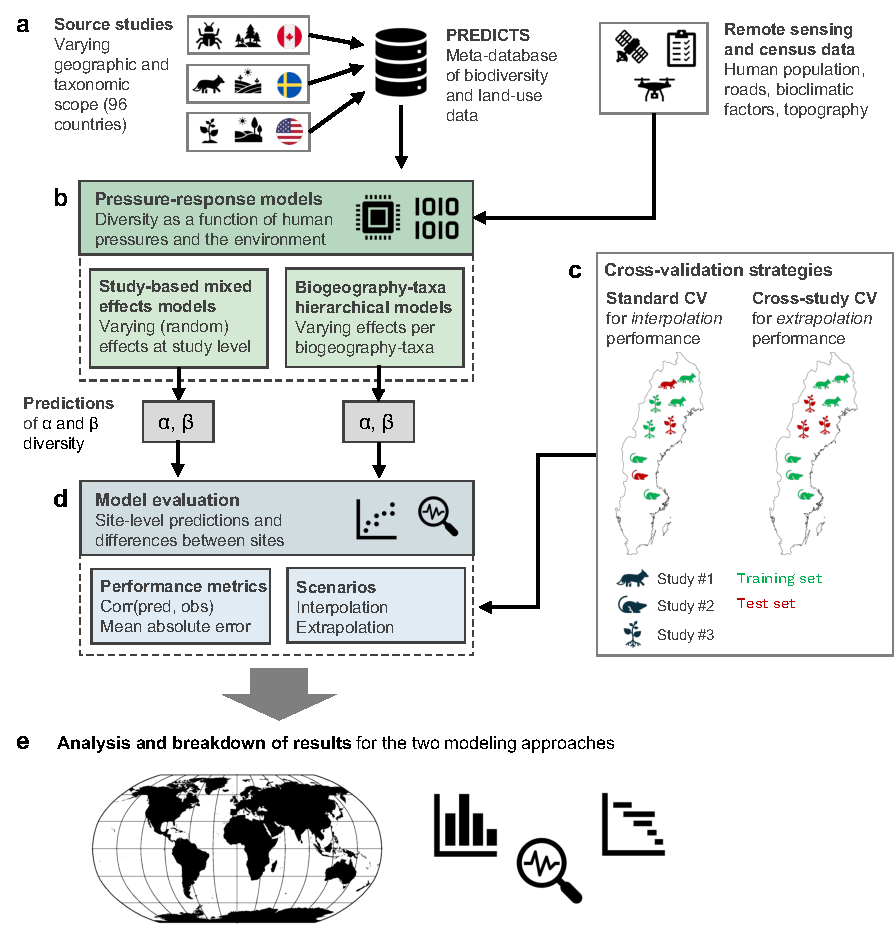
\includegraphics[width=0.96\linewidth]{figures/main/pipeline.pdf}
    \vspace{-10pt}
    \caption{\textbf{Data and model pipeline for this study.}
    \textbf{a}, Biodiversity and land-use data from 681 source studies comprising 25,987 sampling sites were joined with data on human population density, road network density, bioclimatic factors, and topography.
    \textbf{b}, We trained two statistical pressure-response models: 1) A generalized linear mixed effects model with human pressures as fixed effects, where study-level random effects accounted for other variation in the data. 2) A Bayesian hierarchical model with varying parameters at the biogeographic-taxonomic level, also including additional bioclimatic and topographic covariates. Geometric mean abundance was used to represent site-level alpha diversity, while beta diversity was calculated as the Bray-Curtis similarity between ecologically intact reference sites and other sites.
    \textbf{c}, Two cross-validation strategies were used: For interpolation (‘standard’ CV), folds were generated by splitting data at the site level, such that sites from a given study could be allocated to multiple folds. For extrapolation (cross-study validation), folds were based on splits at the study level, such that all sites from a given study only appeared in a single fold.
    \textbf{d}, Model accuracy was assessed through the correlation between predicted and observed values (Pearson’s $r$) and the mean absolute error (MAE).
    \textbf{e}, The results were analyzed to understand performance differences and issues across model types, scenarios and countries.
    \textit{Flag icons source: Freepik (CA, SE), iconset.co (US). Map source: The Transhumanist.}}
    \par\vspace{0pt}\noindent\rule{\linewidth}{0.4pt}
    \label{fig:pipeline}
\end{figure}

global extent and broad taxonomic scope evaluated here. The amplified data limitations that come with this\cite{hughes2021,chapman2024,boyd2023} makes evaluation more challenging\cite{depalma2021} but nonetheless important\cite{martin2019}. To our knowledge, this has not been done for pressure-based biodiversity models with a global scope.

Here we quantitatively evaluate the generality of two different pressure-response models for projecting site-level biodiversity (overview in \autoref{fig:pipeline}). Generality is operationalized as model accuracy when making spatially explicit, out-of-sample predictions in sampled ecological contexts (generalizability) as well as in other contexts (transferability). We leverage species inventory data from 25,987 sites in 96 countries, with broad taxonomic coverage. The data originates from 681 studies collated in the widely used PREDICTS database\cite{hudson2017} (see \autoref{fig:predicts_data}). The first model uses a mixed effects structure\cite{harrison2018} with human pressures as fixed effects, estimated on average across all sites, and random effects to account for variation between studies. Such model structures are common in biodiversity meta-analysis\cite{spake2022} and used in different indicators \cite{newbold2015,schipper2020}. In the second model, we group data by biogeographic and taxonomic attributes in a hierarchical structure. Model parameters are estimated individually for each group, while sharing information across. Environmental variables complement the human pressures to create a richer model. The rationale is to learn from more contextual information that can be used for out-of-sample prediction. Our aim is to explore the implications of biodiversity data availability and model design on generality, providing insights for future work on large-scale biodiversity models.

\section*{Results}
\subsection*{Summary of model predictive performance}

We used geometric mean abundance (GMA) \cite{santini2017} to quantify site-level alpha diversity, reflecting the richness, abundance and evenness of a sampled species community (normalized to a common 0--1 scale across studies \cite{depalma2021}). For beta diversity, we calculated the Bray-Curtis (BC)\cite{bray1957} compositional similarity between ecologically intact reference sites -- consisting of minimally used primary vegetation -- and sites with other land-use types within the same study\cite{depalma2021}. The resulting GMA and BC distributions are shown in \autoref{fig:response_data_distr}. While GMA can be highest at any site within a study, the BC similarity is capped at reference site levels, which explains the lower mean and thinner tail of the latter distribution. Based on the data distributions, we assumed a beta likelihood function for both alpha and beta diversity models.

%The inflation of zeros was caused by a mix of true absences and imperfect detection\cite{dorazio2016,wu2015}.

Human pressure variables describing land-use \cite{hudson2017}, population density \cite{gpw2017},
and road network density \cite{groads2013} formed the core of all models (see detailed list in \autoref{tab:variables}). In the first model, these constituted the fixed effects, while study-level random intercepts and slopes accounted for inter-study differences in taxonomic scope, environment, and sampling. Spatial block intercepts further captured intra-study variation where available. The model structure, variable selection, and use of generalized linear mixed models largely followed previous implementations \cite{newbold2015,depalma2021,bevan2024,schipper2020}. In the second model, the hierarchical structure consisted of two levels: data was first grouped by biome and high-level taxonomic group, then subdivided by biogeographic realms to form regional biomes\cite{bevan2024} (see \autoref{fig:hierarchical_groups}). Groups containing at least five studies used group-level parameters for predictions, while smaller groups were 'rolled up' to the level above, to avoid overoptimistic performance metrics. Environmental variables included temperature and precipitation\cite{fick2017}, and elevation and slope\cite{amatulli2018} (see \autoref{tab:variables}). Study and block identifiers were included during training to control for study heterogeneity. Here we used a Bayesian hierarchical model to achieve regularization through weakly informative priors, handle overparameterization in small groups, and leverage statistical strength across groups  \cite{dorazio2016,lemoine2019,gelman2006}.

\begin{figure}[H]
    \centering
    \noindent\rule{\linewidth}{0.4pt}\par\vspace{6pt}
    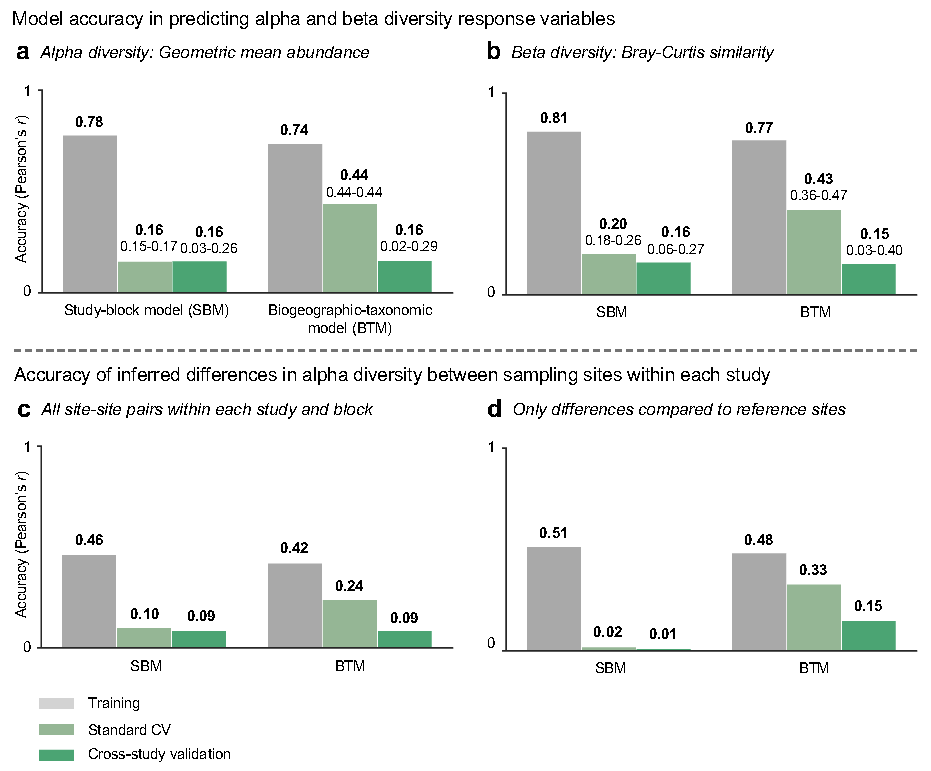
\includegraphics[width=0.95\linewidth]{figures/main/summary_results.pdf}
    \vspace{-10pt}
    \caption{
    \textbf{Summary of model predictive accuracy.}
    \textbf{a–d}, Average predictive accuracy (Pearson's $r$ between predicted and observed values) of the study-block model (SBM) and biogeographic-taxonomic model (BTM). In-sample accuracy on training data is shown in grey, standard cross-validation (CV) accuracy in light green, and cross-study validation accuracy in dark green. For the CV results, the ranges indicate the minimum and maximum accuracies among folds.
    \textbf{a}, Alpha diversity, predictions of site-level geometric mean abundance.
    \textbf{b}, Beta diversity, predictions of Bray–Curtis similarity between pairs of ecologically intact reference sites and other sites, within each study.
    \textbf{c}, Differences in alpha diversity between all site–site pairs within every study and/or block, inferred from the alpha diversity models in (\textbf{a}).
    \textbf{d}, Same as (\textbf{a}) but restricted to pairs containing an ecologically intact reference site.}
    \par\vspace{0pt}\noindent\rule{\linewidth}{0.4pt}
    \vspace{-20pt}
    \label{fig:summary_results}
\end{figure}

A summary of model performance is shown in \autoref{fig:summary_results}. In terms of alpha diversity (\figpanel{fig:summary_results}{a}), the study-block model (SBM, first model above) achieved predictive accuracies of 0.78 on training data, 0.16 in standard cross-validation (CV), and 0.16 in cross-study validation. Accuracy was defined as the Pearson correlation $r$ between observed and predicted values. The corresponding numbers for the biogeographic-taxonomic model (BTM) were 0.74 on training data, 0.44 in standard CV, and 0.16 in cross-study validation. For standard CV, folds were generated using stratified random sampling of \textit{sites} across all studies, to assess generalizability (interpolation accuracy) within sampled contexts. Cross-study validation \cite{bernau2014} evaluated transferability (extrapolation) to other contexts, where each non-overlapping fold contained a stratified random sample of \textit{studies}. For beta diversity (\figpanel{fig:summary_results}{b}) the relative patterns were similar. The accuracies for the SBM were 0.81 (training), 0.20 (standard CV), and 0.16 (cross-study validation); for the BTM they were 0.77, 0.43, and 0.15, respectively. The beta diversity models included the same covariates as described above, plus differences in human population and road density, and the spatial and environmental distance, between sites \cite{depalma2021}. Due to the large number of site pairs in the BC dataset, a sub-sample was used, with inverse weighting based on study size to obtain a more balanced sample.

In addition to the alpha and beta diversity predictions, we looked at estimated and observed \textit{differences} in alpha diversity \textit{within} individual studies and spatial blocks (\figpanel{fig:summary_results}{c,d}), inferred from the predictions in \figpanel{fig:summary_results}{a} (note: these are not separately trained models). The more homogeneous ecological context should provide a more 'level playing field' between the two model structures than \figpanel{fig:summary_results}{a}. When evaluated over all site pairs (\figpanel{fig:summary_results}{c}), the SBM accuracies were at a somewhat lower level than the regular alpha diversity predictions, with standard CV at 0.10 (vs 0.16) and cross-study validation at 0.09 (vs 0.16). The BTM also did worse here, for both standard CV (0.24 vs 0.44) and cross-study validation (0.09 vs 0.16). Finally, we repeated the analysis but restricted to pairs containing reference sites (\figpanel{fig:summary_results}{d}). The inferred site-site differences from the SBM were less accurate than those calculated for all site pairs, yet the opposite was true for the BTM model. It is not clear why that is the case, and since \figpanel{fig:summary_results}{c,d} are not based on a separately trained model, the results should be interpreted with some caution.

\vspace{\baselineskip}

\subsection*{Implications of structural model differences}

The results above reveal notable gaps between in-sample and out-of-sample predictions, with three things standing out: i) The consistently low SBM accuracies; ii) the relatively higher BTM interpolation accuracies (although still quite low in absolute terms); and conversely,  iii) the lack of increase in BTM extrapolation performance. Observation i) is clearly illustrated when comparing the SBM in-sample predictions in \figpanel{fig:lmm_alpha_deepdive}{a} to the out-of-sample results in \figpanel{fig:lmm_alpha_deepdive}{b,c}; predictions were more or less ‘flat’ across all observed values. One key explanation is the low attribution of variance explained\cite{nakagawa2013} to the observable fixed effects (human pressures), relative to the random effects for studies and within-study spatial blocks (\figpanel{fig:lmm_alpha_deepdive}{d}). Since cross-validation simulates model performance on previously unseen sites, the random effects cannot be used when making out-of-sample predictions. The high cross-study heterogeneity around the mean fixed effects (\figpanel{fig:lmm_alpha_deepdive}{e}) further highlights the challenge of model generalization and transferability. Still, as expected from previous studies\cite{keck2025,jaureguiberry2022,newbold2015,depalma2021,bevan2024}, almost all land-use types had negative \textit{average} estimated effects on biodiversity compared to minmally used primary vegetation. The impacts of population and road density were more ambiguous, possibly because these data are static.

The higher BTM interpolation accuracy arose from a combination of model structure -- a biogeographically and taxonomically explicit hierarchy with group-level parameters -- and a richer covariate set. We indeed expect differentiated responses to drivers between groups, and this structure enables generalization of such patterns, assuming that the underlying data is reasonably representative. Further, the richer covariate set was beneficial for predicting alpha diversity across observations globally (\figpanel{fig:summary_results}{a}), where relative distribution patterns depend on environmental factors as well as human pressures, even when data have been normalized. It also helped for beta diversity (\figpanel{fig:summary_results}{b}), since compositional similarity, within the context of a single study, is a function of both human pressures and natural species turnover. The advantage of group-varying parameters also applied when estimating relative levels of alpha diversity within studies and spatial blocks (\figpanel{fig:summary_results}{c,d}). However, there was substantial variation in the average interpolation accuracy between different biogeographic-taxonomic groups, shown for the alpha diversity model in \figpanel{fig:bhm_alpha_groups}{a}, ranging from a few negative values to values close to 0.75. To investigate potential causes of variation, we regressed the group-level accuracies on data attributes of each group (\figpanel{fig:bhm_alpha_groups}{c}). We found that the number of underlying studies and the multivariate Gower distance

\begin{figure}[H]
    \centering
    \noindent\rule{\linewidth}{0.4pt}\par\vspace{6pt}
    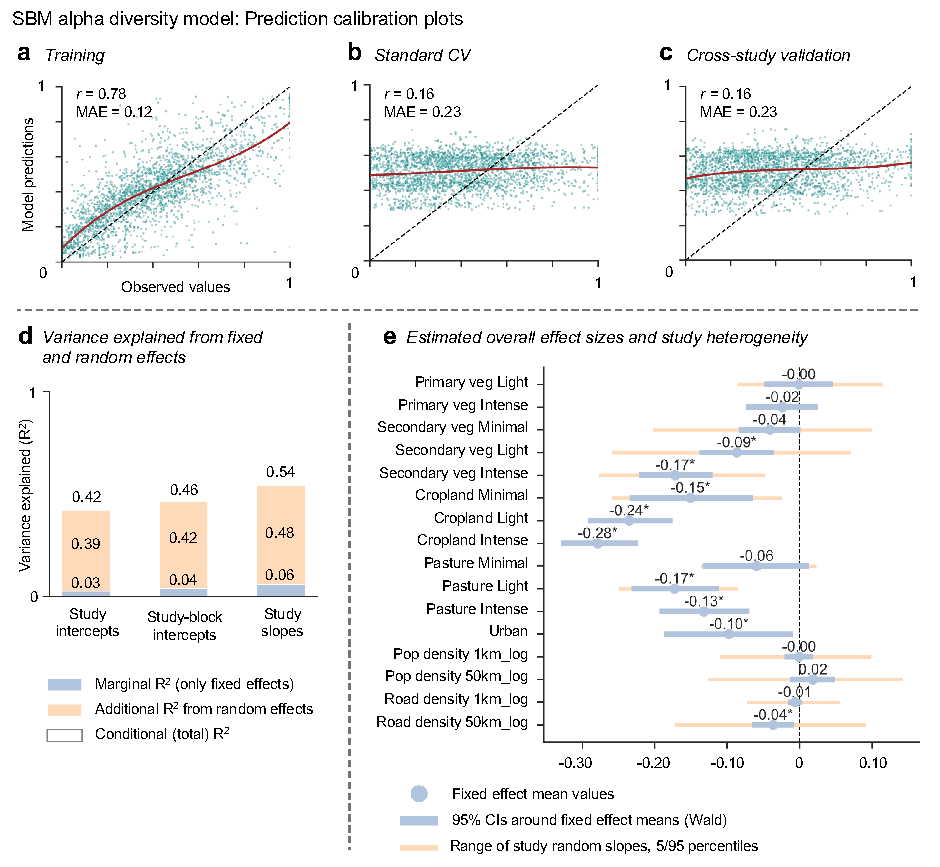
\includegraphics[width=0.95\linewidth]{figures/main/lmm_alpha_deepdive.pdf}
    \vspace{-10pt}
    \caption{
    \textbf{SBM deepdive.}
    \textbf{a}-\textbf{c}, Prediction calibration plots for the SBM alpha diversity model (showing a 10\% random sample for visual clarity), for training data (\textbf{a}), standard CV (\textbf{b}) and cross-study validation (\textbf{c}). The black dashed lines indicate a perfect correlation, whereas the red solid lines show the best polynomial fit to the data.
    %Areas where the solid line is above the dashed line indicate overbiased model predictions, and vice versa.
    \textbf{d}, Decomposition of variance explained between predictions using only the fixed effects (marginal $R^2$, light blue) and predictions including random effects (incremental contribution to conditional $R^2$, yellow). Total variance explained (conditional $R^2$) is shown on top of the bars.
    \textbf{e}, Estimated model parameters. Blue circles show the fixed effect means (across all studies), with blue bars representing 95\% confidence intervals around the mean values. The yellow bars indicate study heterogeneity, the spread of study-level random effects (5–95th percentiles among all studies). Random slope support is uneven across studies, so these estimates are approximate.}
    \par\vspace{0pt}\noindent\rule{\linewidth}{0.4pt}
    \vspace{-20pt}
    \label{fig:lmm_alpha_deepdive}
\end{figure}

between the covariates of each observation and its ten nearest neighbors in the same group, had a negative impact on accuracy (both significant at the 5\% level). This suggests that data heterogeneity negatively impacted performance. On the other hand, the number of taxonomic orders sampled and the standard deviation of the response variable were associated with higher accuracy. One possible interpretation is that the latter captured sampling extensiveness and intensity (together with number of sites, which was positive but not significant), once the aforementioned sources of heterogeneity had been accounted for. However, despite the relative improvement over the SBM, the BTM had clear calibration issues: it overestimated predictions

\begin{figure}[H]
    \centering
    \noindent\rule{\linewidth}{0.4pt}\par\vspace{6pt}
    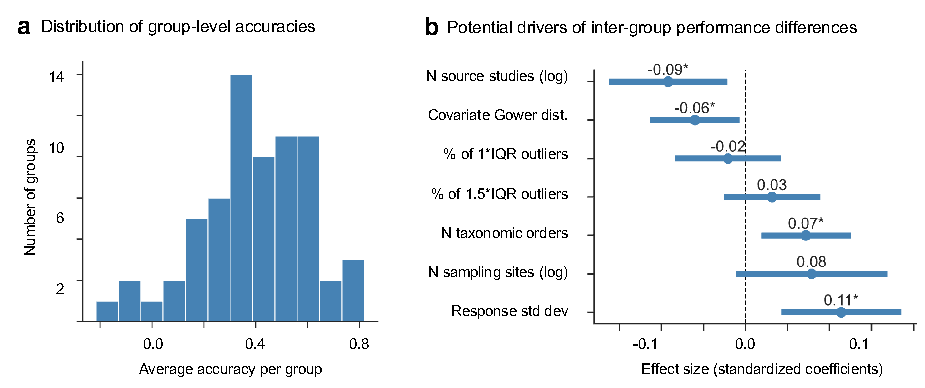
\includegraphics[width=0.95\linewidth]{figures/main/bhm_alpha_groups.pdf}
    \vspace{-10pt}
    \caption{
    \textbf{BTM interpolation deepdive.}
    \textbf{a}, Distribution of group-level average accuracy values of the 60 hierarchical groups included in the BTM model.
    \textbf{b}, Coefficients from linear regression model with group-level accuracy as response variable and data attributes of each group as covariates. All covariates have been standardized to make effect sizes comparable. These should be interpreted as the percentage point change in accuracy from a standard deviation increase in the variable. The bars represent 95\% confidence intervals. The variables are, from top to bottom: The number of source studies in the group (log transformed); the median Gower covariate distance between each observation and its ten nearest neighbors in the same hierarchical group; the proportion of outlier response values (GMA) falling outside of the IQR and 1.5*IQR, respectively; the number of taxonomic orders sampled across studies; the total number of sampling sites (log transformed); the standard deviation of the response variable.
    } \par\vspace{0pt}\noindent\rule{\linewidth}{0.4pt}
    \vspace{-20pt}
    \label{fig:bhm_alpha_groups}
\end{figure}

for small observed values, and vice versa (\figpanel{fig:bhm_alpha_distr_shifts}{b}). This is partially related to the skewness of the response variables (\autoref{fig:response_data_distr}), which is hard to model, but also points to potential bias from latent variables and complex interaction effects.

It should be noted that the structural differences between the models imply some limitations on direct intercomparison. In the SBMs, recall that the fixed effects were estimated based on data from all sites, covering the full spatial and taxonomic scope of the data. The site-level predictions, generated by applying those parameters to local human pressures, were then evaluated against site-level observed values that, naturally, represent a very small share of the full ecological scope of the data. In the absence of taxonomically complete validation data covering major biogeographic regions, this is still a useful approximation. The BTMs, on the other hand, were based on data where the response variables were split by broad taxonomic group. That makes evaluation of predictions more specific to each biogeographic-taxonomic context. While this is a non-negligible difference, it constitutes the best possible way of evaluating the predictions of both models, given the available data.
\vspace{\baselineskip}

\subsection*{Model extrapolation and country-level results}

The drop in BTM extrapolation accuracy (\figpanel{fig:bhm_alpha_distr_shifts}{c}) compared to interpolation (\figpanel{fig:bhm_alpha_distr_shifts}{b}) was caused by distribution shifts between training and test data, which forced the model to make out-of-distribution predictions\cite{meyer2021,meyer2022}. These shifts become evident when comparing the train-test distribution alignment of covariates between the standard CV and cross-study validation runs (\figpanel{fig:bhm_alpha_distr_shifts}{d,e}). Here we calculated the Gower distance \cite{gower1971} between the covariates of each training and test point and its ten nearest neighbors in the training data. The cross-study folds have a higher

\begin{figure}[H]
    \centering
    \noindent\rule{\linewidth}{0.4pt}\par\vspace{6pt}
    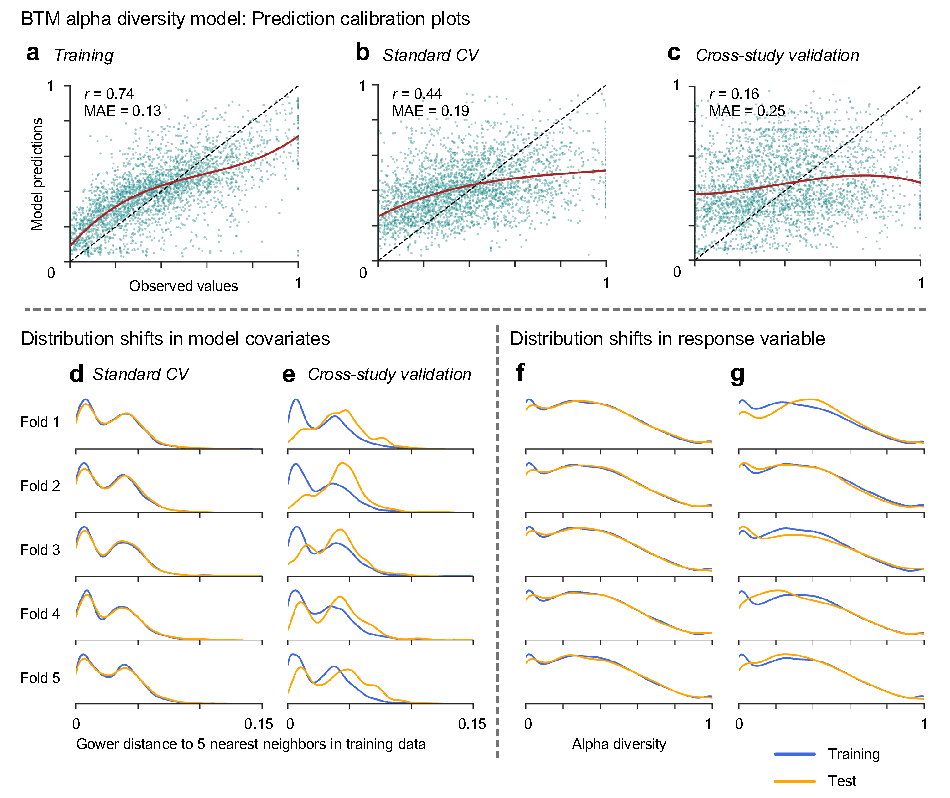
\includegraphics[width=0.95\linewidth]{figures/main/bhm_alpha_distr_shifts.pdf}
    \vspace{-10pt}
    \caption{
    \textbf{BTM extrapolation issues.}
    \textbf{a–c}, Prediction calibration plots for the BTM alpha diversity model (corresponding to the SBM plots in \autoref{fig:lmm_alpha_deepdive}).
    \textbf{d,e}, Distribution density plots obtained by calculating the multivariate Gower distance between the model covariates of each data point, and its hl{five nearest neighbors in the training data (using a sample of 1,000 training points)}. This was done for all training data (blue) and test data (yellow). This gives an indication of how well the joint distribution of covariates align between training and test data in each cross-validation fold, for standard CV (\textbf{d}) and cross-study validation (\textbf{e}).
    \textbf{f,g}, Corresponding density plots of geometric mean abundance of the training and test data in each cross-validation fold, for standard CV (\textbf{f}) and cross-study validation (\textbf{g}).}
    \par\vspace{0pt}\noindent\rule{\linewidth}{0.4pt}
    \vspace{-20pt}
    \label{fig:bhm_alpha_distr_shifts}
\end{figure}

density of test points farther away the training points in covariate space. Some shifts, albeit less pronounced, could be seen for the response variable distributions (\figpanel{fig:bhm_alpha_distr_shifts}{f,g}). At the core, this has to do with model exposure to data. Standard CV involved sampling from a pool of 25,987 sites, such that the model was exposed to a high proportion of the relevant signals in the complete dataset in each fold. In contrast, cross-study validation involved sampling studies from a heterogeneous pool of only 681. This led to a clear spatial, environmental and taxonomic separation of training and test data. Interestingly, although the overall extrapolation accuracies were similar between the two models, the calibration plots (\figrefspanels{fig:lmm_alpha_deepdive}{c}{fig:bhm_alpha_distr_shifts}{c}) show very different patterns. The flexibility of the BTMs, an advantage for interpolation, here led to clear overfitting to the studies seen in training. The SBM, on the other hand, was hampered by the fixed vs random effects issues previously discussed.

The GBF-MF emphasizes country-level reporting of relevant biodiversity indicators \cite{gbfmf2025,affinito2024}. As a complement to the group-level accuracies in \figpanel{fig:bhm_alpha_groups}{b}, we calculated the average accuracy of sampling sites located in each country (\autoref{fig:bhm_country_maps}). We used outputs from the BTM alpha and beta diversity models in the interpolation (standard CV) case. We only included countries with at least two studies and 25 sampling sites, to avoid major outliers skewing the results. The analysis showed large variation in accuracy across countries. This reflects underlying differences in the predictive performance of the models in different biogeographic-taxonomic groups (\figpanel{fig:bhm_alpha_groups}{a}) and the subsets of biogeographic regions, taxa, and sites represented in each country's data (data coverage varies substantially between geographies, see \extfigpanel{fig:predicts_data}{d,e}). Since most country-level datasets are not taxonomically representative, and the need for extrapolation is not factored in, the analysis should be viewed indicatively.

\begin{figure}[tp]
    \centering
    \noindent\rule{\linewidth}{0.4pt}\par\vspace{6pt}
    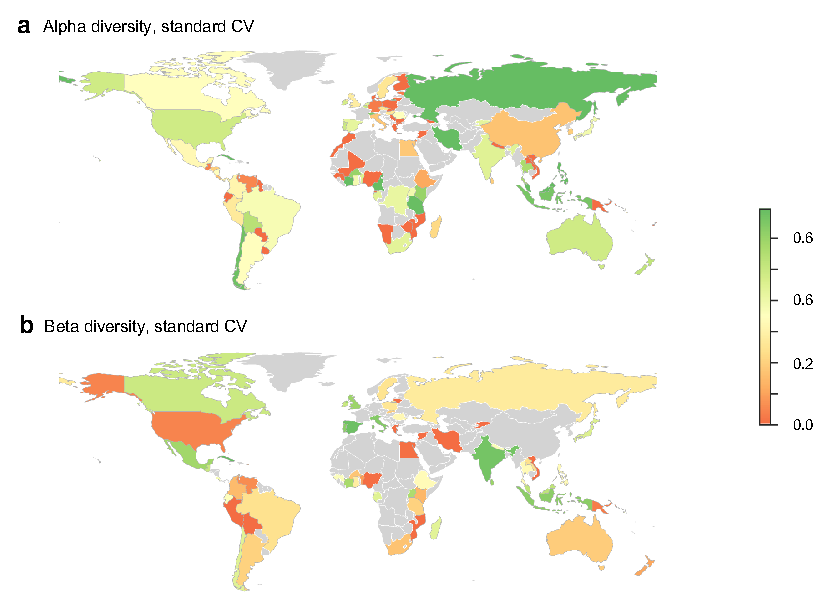
\includegraphics[width=0.95\linewidth]{figures/main/bhm_country_maps.pdf}
    \vspace{-10pt}
    \caption{
    \textbf{BTM accuracy per country.}
    \textbf{a,b}, Average model accuracy calculated per country for the BTM alpha (\textbf{a}) and beta (\textbf{b}) diversity models, when evaluated using standard CV. Only countries with at least two studies and 25 sampling sites are shown. Average accuracy values have been clipped at 0 and winsorized at the 5th and 95th percentiles to prevent outliers from skewing the heatmap gradient. Countries with insufficient data are shown in gray.}
    \par\vspace{0pt}\noindent\rule{\linewidth}{0.4pt}
    \vspace{-20pt}
    \label{fig:bhm_country_maps}
\end{figure}


\section*{Discussion}

In this study, we evaluated the predictive performance of two pressure-based biodiversity models using a global dataset. Our results highlight limits to spatially explicit predictions across models (\autoref{fig:summary_results}), related to data availability and model design. These findings suggest that the generality of large-scale biodiversity models remains a major challenge\cite{spake2022}. Some generalization could be attained within contexts where there was enough data (\autoref{fig:bhm_alpha_groups}), but transferability to new contexts remains elusive (\autoref{fig:bhm_alpha_distr_shifts}). This aligns with prior results at smaller spatial and taxonomic scales\cite{roberts2017,meyer2021,meyer2022}. Given the demand for global biodiversity indicators\cite{burgess2024}, the systematic assessment presented here fills an important knowledge gap. Our results have implications for the use and interpretation of pressure-based models and indicators. These insights can support data collection and model development efforts to further strengthen the critical role of biodiversity models for global policy and decision-making \cite{zurell2025, purvis2025}.

By comparing two structurally different models, we are able to shed light on different aspects of the model generality challenge. Lingering data gaps and biases on a global level \cite{hughes2021,chapman2024} puts fundamental constraints on large-scale biodiversity models. This challenge is clearly shown by the decrease in predictive performance of the BTMs between interpolation and extrapolation (\figpanel{fig:summary_results}{a,b} and \figpanel{fig:bhm_alpha_distr_shifts}{b,c}). The data distribution shifts (\figpanel{fig:bhm_alpha_distr_shifts}{d,e}) that forced the models to make out-of-distribution predictions cannot be adequately addressed without additional data. More representative data implies fewer places where extrapolation is required, and would also enable interpolation within increasingly relevant contexts. To illustrate the second point, consider that the parameters in the BTMs were at the level of 'birds in moist broadleaf forests of the Neotropics', which implies averaging over a great deal of underlying differences in distributions and responses to pressures. Indeed, we saw large variation in performance between hierarchical groups (\figpanel{fig:bhm_alpha_groups}{a}) and across countries (\autoref{fig:bhm_country_maps}), related to data availability and heterogeneity.

The results also highlight the role of model design choices. The SBMs had consistently low performance across interpolation and extrapolation (\autoref{fig:summary_results} and \figpanel{fig:lmm_alpha_deepdive}{b,c}). The use of study-level random effects is sensible for estimating average effects of anthropogenic drivers \cite{harrison2018,pinheiro2000}. However, they also prevent generalization, since models attribute signal to variables that are discarded at the prediction stage (\figpanel{fig:lmm_alpha_deepdive}{d}). This underscores that explanatory power is not necessarily an indicator of predictive power\cite{shmueli2010,tredennick2021}. In comparison, the structure and covariates of the BTMs enabled some, albeit limited, generalization (\FigsTwo{fig:summary_results}{}{fig:bhm_alpha_groups}{a,b}). It is not surprising that a model trained using more contextually explicit information is better at predicting relative levels of alpha diversity (\figpanel{fig:summary_results}{a}). But even if the main goal was to differentiate between sites with different pressures within a given ecological context, our results indicate that the BTMs had an advantage due to their varying-group parameters (\figpanel{fig:summary_results}{b,c,d}). All of this naturally hinges on data being reasonable representative in the biogeographic-taxonomic groups modeled. This is unlikely to be the case everywhere, especially in groups with fewer observations. Still, this hierarchical structure provides a dynamic mechanism for capturing the benefits of increasing data across contexts. Although something similar could be achieved by training separate SBMs per group, it would be less dynamic and not leverage the full data as effectively. For spatial prediction, we argue that it is generally preferable to explicitly model both the natural and anthropogenic factors at play. It should also be noted that our goal was to give an illustrative comparison between the two modeling approaches, not exhaustively optimize performance; that would have involved using more extensive biodiversity, environmental, and anthropogenic data.

Scientifically robust indicators are essential for achieving the goals of the GBF \cite{affinito2024,gbfmf2025}. Global implementations are appealing because they are readily applicable and offer promises of consistency\cite{ipbes2019}. Our results corroborate that, on average, land-use change is a strong driver of biodiversity loss (\figpanel{fig:lmm_alpha_deepdive}{e}), in line with many previous analyses \cite{keck2025,jaureguiberry2022,newbold2015,depalma2021,bevan2024}. Yet, the low model accuracies emphasize the challenging gap between effect size inference and spatially explicit predictions. Maps where spatial resolution is not matched by predictive power can incur concrete risks, such as suboptimal conservation priorities or inaccurate sustainability reports. To effectively support decision-making, the limitations of model-based indicators must be transparent to users. Countries with extensive data can overcome certain limitations by implementing their own models and indicators\cite{gbfmf2025,affinito2024}. However, that would still leave data-poor regions with a lack of accurate biodiversity insights on local scales\cite{clements2025}. Here, resources must be allocated to scale up collection of standardized biodiversity data in prioritized areas and taxonomic groups\cite{hughes2021,gonzalez2023}, leveraging cost-effective technologies like environmental DNA, bioacoustics and camera traps. Similarly, companies that want to ensure accurate decision-making and reporting will often need to collect proprietary data to complement existing tools\cite{goodsell2025}.

%One motivation behind this study was the use of pressure-based models for spatial projections\cite{newbold2015,schipper2020} despite lack of systematic testing\cite{martin2019}.

%In other words, the gap between directional signals and precise estimates can be large.

Our study highlights several research priorities for improving large-scale, predictive biodiversity models. There are clear opportunities to build dynamic and scalable data pipelines that combine large quantities of sampling event data from repositories like the Global Biodiversity Information Facilitaty (GBIF), with the latest remote sensing data from platforms like Google Earth Engine. Contributions of structured sampling data to central repositories should be prioritized, where large-scale datasets are of particular value. More effort should be invested into methodological development of top-down community models, like the ones used in this study, as a complement to species distribution models (SDMs). By aggregating biodiversity data first and then training models, they offer necessary scalability for global applications. Methods that tackle data-sparse contexts and explore the limits of extrapolation are other important avenues of research. Finally, evaluating biodiversity models with such a large scope is a very complex task, and limitations to site-level evaluation and model intercomparison have been highlighted already. This points to the need for evaluation frameworks that can handle scale in multiple dimensions, to assess whether a large-scale model is 'good enough' in a certain context, as opposed to more locally adapted models.

%In conclusion, models are essential for biodiversity monitoring, but our findings demonstrate that the predictive power of pressure-based models has clear limitations. Users need to be aware of these limitations, and the scientific community should prioritize the mobilization of data and development of refined models, to ensure that large-scale biodiversity indicators can reliably guide conservation efforts.

\newpage

% Methods

\section*{Methods}

\subsection*{Data sources}

\textit{Biodiversity data:} All biodiversity data -- species presence or absence, and abundance -- were obtained from the Projecting Responses of Ecological Diversity in Changing Terrestrial Systems (PREDICTS) project \cite{hudson2017}, a meta-database compiled from independent source studies and inventories. We combined the two publicly available releases of the database (from 2016 and 2022) \cite{hudson2023,contu2022} into one dataset. Before filtering (see further down), the combined dataset contained data from 817 studies comprising 35,736 sampling sites in 101 countries, with 4,318,808 unique records across 53,925 species, collected between 1984 and 2018. The PREDICTS data mainly covers animals and plants, with the most common groups being insects and other arthropods, vascular plants, and vertebrate animals. Despite efforts to balance the data taxonomically, vertebrates are over-represented relative to their true diversity, while fungi and non-arthropod invertebrates are underrepresented. Geographically, the dataset has gaps in line with most biodiversity data sources; high-income regions like North America and Europe are well-sampled relative to their underlying biodiversity, some tropical areas in Latin America also have high coverage, while there are significant gaps in Africa and parts of Asia (see \autoref{fig:predicts_data} for an overview of PREDICTS data coverage). In 255 of the source studies, spatially adjacent sampling sites had been grouped into spatial blocks, which was utilized for model training.

\textit{Human pressure data:} The predominant land-use type and land-use intensity at each sampling site has been categorized by the PREDICTS team based on information in the source studies \cite{hudson2017}. Land-use categories include primary vegetation, secondary vegetation (split into young, intermediate, mature, or indeterminate age), plantation forest, cropland, pasture and urban, while use intensity has been classified as minimal, light or intense. Data on human population density, expressed as the number of people per 1~km$^2$, came from the Gridded Population of the World, v4.11 (GPWv4.11) dataset \cite{gpw2017}, based on the 2010 round of Population and Housing Censuses (conducted 2005--2014) and adjusted to match the United Nations World Population Prospects country totals. The population data represents extrapolated numbers for the years 2000, 2005, 2010, 2015, and 2020.  Data on road networks were taken from the Global Roads Open Access Data Set, v1 (gROADS) \cite{groads2013}, a global layer of joined country road networks adjusted for topology. Data were collected between 1980 and 2010, with limited information on original road construction dates.

\textit{Bioclimatic and topographic data:} Bioclimatic variables, such as annual averages, seasonality and extreme values of temperature and precipitation, were based on the WorldClim v2.1 dataset\cite{fick2017}, frequently used in species distribution models and other biodiversity studies. The data represent average values over the period 1970--2000. Data on elevation, slope and terrain roughness came from the EarthEnv repository \cite{amatulli2018}, constructed from global digital elevation models derived from satellite imagery and LiDAR measurements.

The spatial resolution of the PREDICTS land-use data depends on the specific sampling extent of a given site in each source study \cite{hudson2017} (which is only available for 13.1\% of sampling sites). The resolution of the population density, bioclimatic and topographic variables is 30 arc-seconds (approximately 1~km$^2$ at the equator) \cite{gpw2017,fick2017, amatulli2018}. The spatial accuracy of the road network data varies by country\cite{groads2013}. Manual classification of land-use type and intensity could have introduced inconsistencies within and between studies \cite{hudson2017}. Since predominant land-use is a categorical attribute, there might be underlying differences in habitat conditions within the same class that are notn observed. The remote sensing and census data layers are all modeled to some extent, potentially introducing additional uncertainty and errors.
\vspace{\baselineskip}


\subsection*{Biodiversity metrics}

We modeled two biodiversity metrics, the geometric mean abundance (GMA) \cite{santini2017}, an alpha diversity metric, and the Bray-Curtis (BC) similarity \cite{bray1957}, a beta diversity metrics. Combined, they provide insights into the relative level of community richness, abundance, evenness, and compositional similarity between areas, and are suitable for detecting changes in biodiversity \cite{santini2017}. If we let $a_{si}$ represent the population abundance of species $s$ at sampling site $i$, and let $S_i$ represent the total number of species at the site, the GMA of that site can be calculated as
\vspace{0.25\baselineskip}
\begin{equation*}
    y_i = \exp\left(\frac{\sum_{s=1}^{S_i} \ln a_{si}}{S_i}\right).
\end{equation*}

The ln transformation dampens the contribution of highly abundant (perhaps generalist or opportunistic) species. For a given total site abundance, higher species richness and evenness results in a greater GMA. For beta diversity, the BC similarity between two sampling sites $i$ and $j$ is given by
\vspace{0.25\baselineskip}
\begin{equation*}
    y_{ij} = \frac{2\sum_{s=1}^S \min(a_{si},a_{sj})}{\sum_{s=1}^S \big(a_{si}+a_{sj}\big)},
\end{equation*}

where $S$ represents the total number of species found at any of the sites. This is equivalent to an abundance extension of the Sørensen index. The index takes a value of 0 if there are no shared species between sites $i$ and $j$, and a value of 1 if the species and their abundances are identical between the two sites (which is highly unlikely). Since the focus of this study is on models used to estimate biodiversity intactness, the BC similarity is calculated between reference sites, consisting of minimally used primary vegetation sites, and all other sites within each study. This follows the approach used in the BII\cite{depalma2021} and is similar to the implementation of MSA in GLOBIO \cite{schipper2020}.

\vspace{0.25\baselineskip}
One challenge with biodiversity meta-databases is that the abundance distributions from different source studies will be greatly influence by taxonomic scope, biogeographic area and sampling method. Furthermore, while abundance is often expressed as a count of individuals, it can also be a proportion or density. The most viable approach we found, following the BII \cite{depalma2021}, was to normalize the GMA values within each study to a common 0--1 scale, by dividing them by the respective within-study maxima:
\begin{equation*}
    y_i^{\text{norm}} = \frac{y_i}{\max(y_1,\ldots,y_I)}.
\end{equation*}

The BC index is already expressed on a 0--1 scale, so no further processing was needed. For simplicity, we let $y_i$ denote the normalized values from hereon. Although the sampling method is consistent between sampling sites within a given source study, sampling effort between sites can vary, so effort-adjusted abundance numbers (already provided in the PREDICTS data) were used in all analyses. Since both diversity metrics require abundance data, we filtered out studies that only recorded presences and absences. To mitigate the impact of extreme abundance values, we identified outlier locations using the interquartile range (IQR) method and removed site-level observations where $y_i > 1.5 \,\text{IQR}$, within each study.

The distributions of the alpha diversity (GMA) and beta diversity (BC similarity) metrics are shown in \autoref{fig:response_data_distr}. They are non-symmetric and quite heavily skewed to the right. The shapes are similar, but the GMA distributions have greater means than the BC indices, since a compositional similarity metric to a greater extent reflects natural species turnover across the landscape. There is an inflation of zeros in both distributions, and an inflation of ones in the GMA data. A site-level abundance of zero can either be the result of true absence of the surveyed species, or the result of imperfect detection, a well-known issue in biodiversity data. In the best case, noise that arises from imperfect detection is randomly distributed across studies and sites, but we acknowledge that there could be more systematic detection biases in the data. In addition, studies that only surveyed a small number of species are more likely to have zeros at the site level. However, there is no feasible way to construct a separate detection probability model \cite{dorazio2016,wu2015} for such a heterogeneous dataset using the data that we have available. The inflation of zeros in the BC distribution is the result of a mix of observed zero abundances and complete dissimilarity in species composition between sites. The inflation of ones in the GMA data is an artifact of the normalization procedure described above, since every study will contribute a one (its maximum abundance site) to the overall data pool.

In the main results, we used data from all studies except for what was subject to the filters described above (such as requiring abundance data). It should be noted, however, that one issue is that many source studies contain very few sites: 18.8\% contain 5 sites or less, and 60.9\% contain 25 or fewer (see \autoref{fig:sites_per_study}). There is a risk that such small studies contribute more noise than signal to the overall pool of data used to train the models. Informally, this is because there are not enough observations from the context of a given study to reliably relate its species observations to different human pressures and environmental conditions. Through inspection of study-level histograms, we found that ideally 25--50 sites per study would be required to produce somewhat continuous distributions of data at the study-level. Some of this is alleviated by pooling data across studies, but some biases can certainly persist.

%This is supported by the fact that a threshold of 25 sites when training and evaluating the BHM resulted in better model performance than no threshold or a 10-site threshold (\hl{Extended Data Fig. X}). We still chose to include all data as the aim of the study was to illustrate the current state of model performance using available data, not optimizing for accuracy.

The biogeographic-taxonomic models (BTMs) used taxonomic groups as part of the hierarchical model structure (see \autoref{fig:hierarchical_groups}). Since some larger studies had sampled species across several such taxonomic groups, sampling sites were consequently split into multiple observations (compare \extfigpanel{fig:response_data_distr}{c,d} to \extfigpanel{fig:response_data_distr}{a,b}). The BTM alpha model had 31,242 observations in total, in comparison to the 25,987 sampling sites in scope, which also equaled the number of observations in the study-block model (SBM). Since the BC similarity dataset contained more than 400,000 unique site pairs after standard filtering, we used sub-sampling to obtain a tractable but representative dataset for model training and evaluation. The sampling was designed to retain all studies with at least one reference site, while preventing large studies, with many sites and reference sites, from becoming too dominant. For each study $s$, we calculated the number of potential pairs $n_{sites} \times n_{ref}$ and a sublinear weight $w_s = \sqrt{n_{sites} \times n_{ref}}$, with $w_{tot}$ denoting the sum of all study weights. An initial number of pairs was allocated to each study based on its actual number of pairs $n_{pairs}$ and an overall target fraction $f  = 0.10$ of the whole dataset. This was weighted by $w_s$ and subject to lower and upper bounds $k_{min}, k_{max}$, such that $k_s = \text{max}(k_{min}, \text{min}(n_{pairs} \times f \times w_s / w_{tot}), k_{max})$. The threshold values were set to $k_{min} = 300$ and $k_{min} = 3,000$, respectively, to increase the contribution of smaller studies and limit the dominance of the largest ones. To balance reference sites and other sites within each study sample, we finally chose $\sqrt{k_{study}}$ non-reference sites and $k_{study} / \sqrt{k_{study}}$ reference site, to get approximately $k_{study}$ sites in total. This resulted in a total of 29,088 site pairs that were consistent across SBM and BTM models.
\vspace{\baselineskip}


\subsection*{Data likelihood function}

The GMA and BC distributions are non-symmetric and bounded between 0 and 1, with substantial inflation of zeros and some inflation of ones in the GMA case (\autoref{fig:response_data_distr}. This suggests that a zero-inflated or zero-one-inflated beta distribution would be the most appropriate likelihood function to describe the data \cite{ospina2010}. The beta distribution is 0-1 bounded and can have a more or less symmetrical shape depending on its parameters. However, since our goal was to predict biodiversity on highly aggregated levels, it seemed counterproductive to explicitly model the zero-inflation, as true absences of entire species groups in a given area are unlikely. Further, the inflated ones are scaling artifacts (due to the inter-study normalization) that did not warrant explicit modeling either. We therefore assumed a regular beta likelihood function, with a logit link function, for all models \cite{ferrari2004}. Further information about how this was implemented can be found in the modeling sections below.

\vspace{\baselineskip}

%During initial testing of the BTMs, we compared the results of a regular beta distribution against a Gaussian likelihood, the latter representing a simplified assumption about the data generating process. Although the shapes of the beta posterior distributions were more similar to the observed data, compared to its Gaussian counterpart, the predictive accuracy of the Gaussian models were generally higher. Since the aim of the study was to benchmark predictive performance, and Gaussian models are computationally simpler, with more interpretable model coefficients, we decided to use Gaussian likelihood functions across all models.


\subsection*{Model covariates}

Variables based on land-use \cite{hudson2017}, population density \cite{gpw2017}, and road network density \cite{groads2013} data, formed the core of all models in the study\cite{depalma2021}. For land-use, the land-use class and its intensity was combined into a new set of categorical variables; records where this information was unknown were filtered out. Minimally used plantation forest was grouped with lightly used secondary forest, and other plantation forest (light and intense use) was grouped with intensely used secondary forest \cite{depalma2021}. The categorical land-use variables were one-hot encoded, with the model intercepts representing minimally used primary vegetation reference sites. Human population density and road network density at 1 and 50~km$^2$ scales, log transformed to reduce skewness, were also part of all models. The BTMs additionally included the following bioclimatic and topographic variables: annual mean precipitation and temperature (1~km$^2$), temperature and precipitation seasonality (1~km$^2$), elevation (1 and 10~km$^2$), and terrain roughness (1 and 10~km$^2$). A complete list of model covariates can be found in \autoref{tab:variables}. We did not include any interaction effects due to the small number of observations in many studies (and to some extent, hierarchical groups), implying that the models were already highly parameterized, and even overparameterized to some extent, given the variables above (see \autoref{fig:sites_per_study} for data coverage and below for a discussion on implications of this).

To derive the continuous variables, the coordinates of each sampling site were first projected from global EPSG:4326 to local UTM format, before generating circular polygons of different spatial extents. The equal-area projections ensured that the calculated values were comparable across all locations, regardless of distance to the equator. For each raster dataset (human population density, bioclimatic, topographic) the mean value of each polygon was calculated (including partially covered pixels), after which the polygons were reprojected to the global format. For the road network data, a similar approach was used to derive road density as the combined length of all roads within each polygon. Population density data were interpolated between the available years in the GPW dataset, and back to the earliest PREDICTS data (1984), assuming an exponential growth rate \cite{goldewijk2005}. The population densities were matched to the sampling year of each site; the other covariates were static layers.

For the beta diversity (BC) models, we used the alpha diversity model covariates as a starting point. Here, the land-use variables described the conditions at the non-reference site in each pair, since the reference sites constitute the model intercepts (minimally used primary vegetation). Differences in the human population and road density variables were calculated for each site pair. Additionally, the spatial (Haversine) distance, and multivariate environmental (Gower) distance \cite{gower1971}, were included to control for natural compositional turnover \cite{depalma2021}. The Haversine distance was normalized by the median sampling extent among all studies. The Gower distance was calculated using the following variables, all at the 1~km$^2$ scale: maximum and minimum temperature of the warmest and coldest months, respectively, precipitation of the wettest and driest months, and elevation. All continuous variables were standardized prior to model training, and evaluated for collinearity within their respective category.
\vspace{\baselineskip}


\subsection*{SBMs: Generalized linear mixed models}

The SBMs were implemented as generalized linear mixed models (GLMMs), using the R package \texttt{glmmTMB} \cite{mcgillycuddy2025}. The model structure consisted of fixed effects, parameters representing average values over all studies in the dataset, and random effects, which quantify group-level variation around the fixed effects \cite{harrison2018,pinheiro2000}. The study-level random intercepts and slopes accounted for inter-study differences in geographic and taxonomic scope, environment, and sampling. For studies that grouped spatially adjacent sites into blocks, corresponding intercepts were included to capture intra-study differences. Since all site-level species observations were aggregated to form the response variables, the fixed effects were estimated as an average of all geographies and taxa in the data\cite{newbold2015,newbold2016,depalma2021}.

We let $\boldsymbol{\beta}$ denote the fixed effects and let  $\boldsymbol{\gamma}_s$ denote the study-level random effects, for the study $s$ that site $i$ belongs to. The spatial block intercepts are denoted by $\gamma_{sb(s)}$ for each block $sb$ within study $s$. These different effects constitute a hierarchical structure, from the population of all studies to individual source studies, and from studies to blocks. As noted above, we used a beta likelihood with a logit link function $g(\cdot)$ across all models\cite{ferrari2004}. The mean of $y_i$, conditional on the covariates, is denoted by $\mu_i$. The site-level regression model for GMA can then be written as
\vspace{0.25\baselineskip}
\begin{equation*}
    g(\mu_{i}) = \mathbf{x}_i^\top \boldsymbol{\beta} + \mathbf{x}_i^\top \boldsymbol{\gamma}_s + \gamma_{sb(s)} = \eta_i,
\end{equation*}

where $\mu_i = g^{-1}(\eta_i) = e^{\eta_{i}} / (1 + e^{\eta_{i}})$. We fitted a full set of random slopes at the study level, such that the random effect covariates are the same as the fixed effect ones $\mathbf{x}_i$. The $\boldsymbol{\gamma}_s$ parameters are assumed to be uncorrelated and vary around the fixed effects with mean zero and diagonal covariance matrix $\boldsymbol{\Sigma}_{\gamma}$, such that $\boldsymbol{\gamma}_s \sim \mathcal{N}(\bf{0}, \boldsymbol{\Sigma}_{\gamma})$. The variance of the beta distribution, which is dependent on the conditional means, is given by
\begin{equation*}
    \text{Var}(y_i | \mu_i, \phi) = \frac{\mu_i(1 - \mu_i)}{1 + \phi}.
\end{equation*}

The dispersion parameter $\phi$ was assumed to be constant across studies and observations. In the beta diversity model, $y_{ij}$ denotes the BC similarity between some site $i$ and a reference site $j$, within the context of a study $s$. In addition to the regular covariates $\mathbf{x}_i$ for the non-reference site, we let $\mathbf{z}_{ij}$ denote the set of delta measures calculated between the two sites: the difference in the population and road density, the spatial distance, and the environmental distance. If we let $\boldsymbol{\beta}^\Delta$ and $\boldsymbol{\gamma}_s^\Delta$ denote the parameter vectors associated with these difference terms, we can write the beta diversity model as
\vspace{0.25\baselineskip}
\begin{equation*}
    g(\mu_{ij}) = \mathbf{x}_i^\top \boldsymbol{\beta} + \mathbf{z}_{ij}^\top \boldsymbol{\beta}^\Delta + \mathbf{x}_i^\top \boldsymbol{\gamma}_s + \mathbf{z}_{ij}^\top \boldsymbol{\gamma}_s^\Delta + \gamma_{sb(s)}.
\end{equation*}

Due to the number of covariates (\autoref{tab:variables}) relative to the amount of sites in the smaller studies (\autoref{fig:sites_per_study}), and that all land-use types and intensities are not present in each study, there were some convergence issues when fitting the random study slopes. To ensure that this did not affect the overall results presented, we refitted the alpha and beta diversity models with a threshold of minimum 25 sites per study. This resulted in somewhat lower accuracies for both models: alpha diversity, training: 0.76, standard CV: 0.14, cross-study validation: 0.09; beta diversity, training: 0.81, standard CV: 0.19, cross-study validation: 0.15. While some convergence issues remained, due to uneven representation of land-use classes, it implies that the overall results are robust.

\vspace{\baselineskip}


\subsection*{BTMs: Bayesian hierarchical models}

The SBM structure was built around the data collection process, with studies that sampled sites which were sometimes organized into spatial blocks. In the BTMs, we instead created the hierarchical structure based on the biome and realm where each site is located, and the taxonomic group(s) that were sampled at that site. This was implemented as a two-level hierarchy. At the first level, biomes were combined with taxonomic groupings. Biomes (e.g. tropical and subtropical moist broadleaf forests) are distinct in their environmental conditions and underlying biodiversity patterns, which suggests that the effect sizes of both natural and anthropogenic drivers will be different between them. The taxonomic groupings were based on differences in spatial distribution patterns\cite{jenkins2015} and potentially differentiated responses to drivers. At the same time, data limitations and taxonomic imbalances implied that most taxa were aggregated at quite high levels. For the second hierarchical level, the biome-taxonomic groups were further subdivided by biogeographic realms (e.g. Neotropics) to form so-called regional biomes\cite{bevan2024}. This results in a structure characterized by parent-child relationship between groups at the first and second hierarchical levels.

Although this model could have been implemented as a frequentist linear mixed model, the Bayesian formulation enabled additional flexibility, stronger borrowing of statistical strength across groups, and regularization through weakly informative priors \cite{dorazio2016,gelman2012,lemoine2019}. Groups with low information content are pulled towards their parent group, while groups with sufficient statistical power are able to deviate from those mean values. Still, note that the main comparison in this study is between the overall model approach and structure, not frequentist versus Bayesian implementations.

We let $b = 1, \dots, B$ denote biomes, $t = 1, \dots, T$ taxonomic groups, and $r = 1, \dots, R$ biogeographic realms. Further, $r(b)$ indicates the partition of a given biome into realms. However, note that realms can span multiple biomes and vice versa, so this is not a unique one-to-one mapping. For the group-level model parameters, intercepts are denoted by $\alpha$ and other parameters by $\boldsymbol{\beta}$. To make observations conditionally independent during training, we also included study-block identifiers $\gamma_{sb(s)}$ as control variables, identical to the random intercepts of the SBM models. These were used in model training but not for any out-of-sample predictions. Like the SBMs, the BTMs assumed a beta distributed likelihood with a logit link function. The alpha diversity (GMA) model for taxonomic group $t$ at site $i$, in the regional biome $r(b)$ can be written as
\vspace{0.25\baselineskip}
\begin{equation*}
    g(\mu_{i,t}) = \alpha_{t,r(b)} + \mathbf{x}_i^\top \boldsymbol{\beta}_{t,r(b)} + \gamma_{sb(s)},
\end{equation*}

where the covariates $\mathbf{x}_i^\top$ are defined at the site level (same for all taxonomic units $t$ at the site). We assumed normal and uncorrelated priors for the model parameters, with half-normal priors on the variance terms. At the population-level, the following hyperpriors were used:
\vspace{0.25\baselineskip}
\begin{equation*}
\begin{aligned}
    \mu_{\alpha} \sim \mathcal{N}(0.35, 0.30^2), \; \mu_{\beta}^{(k)} \sim \mathcal{N}(0, 0.15^2)  \; \text{for} \; k = 1, \dots, K,
\end{aligned}
\end{equation*}

where the $K$ is the number of regression parameters. These priors define distributions over the population-level model parameters, which sit at the very top of the hierarchy. The priors at the first hierarchical level (biome-taxa) were drawn from the hyperpriors in the following way:
\vspace{0.25\baselineskip}
\begin{equation*}
\begin{gathered}
    \alpha: \sigma_{\alpha} \sim \text{Half-Normal}(0.20^2), \; \alpha_{t,b} \sim \mathcal{N}(\mu_{\alpha}, \tau_{t,b} \cdot \sigma_{\alpha}^2) \\
    \beta: \sigma_{\beta} \sim \text{Half-Normal}(0.12^2), \; \beta_{t,b}^{(k)} \sim \mathcal{N}(\mu_{\beta}, \tau_{t,b} \cdot \sigma_{\beta}^2)
\end{gathered}
\end{equation*}

The scaling factor, $\tau_{t,b} = \sqrt{n_{t,b}} -1$, adapted the amount of regularization -- through the prior variance -- on the group-level model parameters as a function of the number of studies in each biome-taxa group. In a similar way, the priors at the second level (biome-taxa-realm) inherited from their respective parent groups at the first level, but with tighter priors on the slope variances:
\vspace{0.25\baselineskip}
\begin{equation*}
\begin{gathered}
    \alpha: \sigma_{\alpha} \sim \text{Half-Normal}(0.20^2), \; \alpha_{t,r(b)} \sim \mathcal{N}(\alpha_{t,b}, \tau_{t,r(b)} \cdot \sigma_{\alpha}^2), \\
    \beta: \sigma_{\beta} \sim \text{Half-Normal}(0.10^2), \; \beta_{t,r(b)}^{(k)} \sim \mathcal{N}(\beta_{t,b}^{(k)}, \tau_{t,r(b)} \cdot \sigma_{\beta}^2).
\end{gathered}
\end{equation*}

The numeric prior values above were chosen based iterative prior predictive checks, to obtain a prior predictive distribution reasonably similar to the observed data (\extfigpanel{fig:response_data_distr}{c}) and achieve a relatively high degree of model regularization. Next, the beta diversity model can be expressed as
\vspace{0.25\baselineskip}
\begin{equation*}
    g(\mu_{ij,t}) = \alpha_{t,r(b)} + \mathbf{x}_i^\top \boldsymbol{\beta}_{t,r(b)} +\mathbf{z}_{ij}^\top \boldsymbol{\beta}_{t,r(b)}^\Delta + \gamma_{sb(s)}.
\end{equation*}

The prior structure was identical to the alpha diversity model, but we assumed slightly different hyperpriors due to the lower mean and longer tail of the BC similarity distribution (\extfigpanel{fig:response_data_distr}{d}):
\vspace{0.25\baselineskip}
\begin{equation*}
\begin{aligned}
    \mu_{\alpha} \sim \mathcal{N}(0.25, 0.25^2), \; \sigma_{\alpha} \sim \text{Half-Normal}(0.15^2).
\end{aligned}
\end{equation*}

Further, the scaling factor used the natural logarithm, $\tau_{t,b} = \text{ln}(n_{t,b}) -1$, since this gave better results. For the dispersion parameter of the Beta likelihood, we sampled a raw scale
parameter $\sigma_{\mathrm{raw}} \sim \mathrm{Beta}(a,b)$, using $a=2,b=12$ for
the GMA model and $a=2,b=20$ for the BC similarity model. We then defined a mean-dependent dispersion
$\sigma(\mu_{i,t}) = \sigma_{\mathrm{raw}} \sqrt{\mu_{i,t}\left(1-\mu_{i,t}\right)}$ and used it to parameterize the beta likelihood:
\begin{equation*}
    y_{i,t} \sim \mathrm{Beta}\!\left(\mu_{i,t}, \sigma(\mu_{i,t})\right).
\end{equation*}

Since many biogeographic and taxonomic groups contained only a few studies and sites (\autoref{fig:predicts_data}), there was a risk that the estimated group-level parameters would become too specific to a few studies, rather than generally applicable to the group at large. To prevent this from producing overoptimistic accuracy numbers, especially for interpolation, we implemented a 'roll-up' scheme for out-of-sample predictions. Here, biome-taxa-realm ($t,r(b)$) groups with less than five studies were assigned the parameters of their respective parent groups at the biome-taxa ($t,b$) level for prediction, such that $\boldsymbol{\beta}_{t,r(b)} := \boldsymbol{\beta}_{t,r}$. If the threshold was still not met at the biome-taxa level, the population-level posterior parameters were used. The BTMs were implemented in \texttt{PyMC} \cite{abril-pla2023}, using the No-U-Turn Sampler (NUTS)\cite{hoffman2014} with a \texttt{numpyro}\cite{phan2019} backend. For all experiments, we ran four parallel sampling chains for stability, using 1,000 tuning samples that were discarded and 1,000 posterior draws. A high target acceptance rate of 0.95 was used to avoid problems when sampling from the complex posterior distribution. Due to the high number of diverse hierarchical groups before roll-up (181), some which are quite small, it was hard to avoid some parameters having small effective sample sizes and $\widehat{R}>1.01$\cite{vehtari2019}. While this could indicate convergence issues in the sampling, the overall performance results were robust also when using much fewer iterations than in the final runs.

\vspace{\baselineskip}


\subsection*{Cross-validation and performance metrics}

We evaluated model generality and performance using two complementary cross-validation (CV) approaches. Five CV folds were used in all model runs, with stratified sampling using biomes as strata. The first approach, using 'standard' CV, assessed how well models could make predictions in environmental and taxonomic contexts similar to the data that they were trained on. In other words, this evaluated model generalizability from sample to sampled population, also referred to as interpolation accuracy. The folds were generated by sampling at the site level among all studies within a given stratum. This implies that sites from a given study were generally split among several folds, creating overlap in studies, but not sites, between folds. In the BTMs, fold assignment was still done at site level, keeping multiple taxonomic units for a given site in the same fold, if present.

The second approach, based on cross-study validation \cite{bernau2014}, was used to assess how well the models could make predictions in new contexts; specifically, whether model learning was transferable between different source studies. In this case, folds were constructed by sampling at the study level, such that all sites from a given study ended up in a single fold. The only exception was if a study spanned several strata (biomes), in which case it could appear in more than one fold. The cross-study validation approach led to a clear spatial and environmental separation of training and test data, while also reflecting taxonomic and methodological differences between source studies. Although the numbers of studies per fold were roughly equal, one consequence of the cross-study procedure was that folds in some iterations became unbalanced in terms of the number of sites, due to the large spread in the size of different studies. In this study we defined model accuracy as the Pearson correlation coefficient between predicted values $\widehat{\mathbf{y}}$ and observed values $\mathbf{y}$:
\vspace{0.25\baselineskip}
\begin{equation*}
    r(\widehat{\mathbf{y}}, \mathbf{y}) = \frac{\text{Cov}(\widehat{\mathbf{y}},\, \mathbf{y})} {\sqrt{\text{Var}(\widehat{\mathbf{y}})} \, \sqrt{\text{Var}(\mathbf{y})}}.
\end{equation*}

We chose the correlation coefficient since it is widely recognized, easy to interpret, and provides a normalized measure of performance (values lie between $-1$ and $1$). It directly relates to the calibration plots in \autorefs{fig:lmm_alpha_deepdive} and \ref{fig:bhm_alpha_distr_shifts}; a well-calibrated model should exhibit a linear relationship between predictions and observations. For the BTMs, $\widehat{\mathbf{y}}$ represent the conditional mean predictions (more comparable to the SBMs, as opposed to the mean of the posterior predictive distribution, which also includes the modeled noise). As a complementary metric, we used the mean absolute error (MAE), defined as
\vspace{0.25\baselineskip}
\begin{equation*}
    \text{MAE} = \frac{1}{n} \sum_{i=1}^n \left| y_i - \widehat{y}_i \right|.
\end{equation*}

Since the response variables were on a 0--1 scale, this metric can be interpreted as the average percentage point deviation between predicted and observed values.

\newpage
\printbibliography
\newpage

\section*{Acknowledgments}

We thank Alice Hughes for feedback on conceptual framing and preliminary results. We also thank Robert Goodsell, Emma Granqvist, Adrian Baggström, Mahwash Jamy, Vun Wen Jie and one anonymous reviewer for reading and providing feedback on the manuscript.

\section*{Author contributions}

JN conceptualized the study and developed the overall approach with support from JRS, LM and TA. JN processed the data, implemented the models, and conducted the statistical analyses. All authors provided continuous feedback on the results. JN wrote the first draft of the paper. All authors edited and approved the final version.

\section*{Code availability}

The code for this study can be found at: \url{https://github.com/j-nystrom/biodiversity-impacts}.

\newpage

\section*{Extended Data}
\vspace{2\baselineskip}

\begin{extendedfigure}[ht]
    \centering
    % Top horizontal rule
    \noindent\rule{\linewidth}{0.4pt}\par\vspace{6pt}
    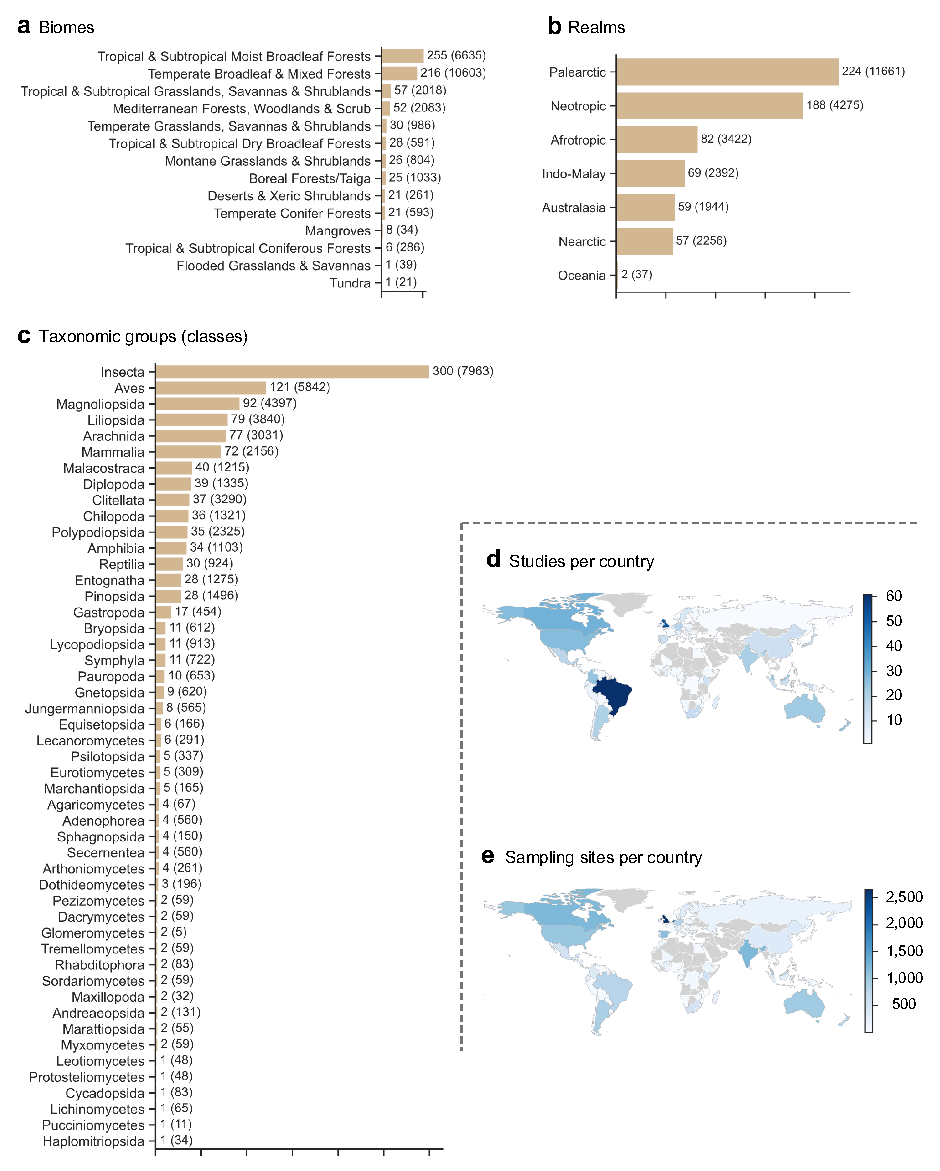
\includegraphics[width=0.95\linewidth]{figures/extended/predicts_data.pdf}
    \caption{
    \textbf{PREDICTS data coverage.}
    \textbf{a-c}, Number of source studies and sampling sites (in parenthesis) in the model data, split by biomes (\textbf{a}), realms (\textbf{b}), and taxonomic classes (\textbf{c}).
    \textbf{a,b}, Number of source studies (\textbf{a}) and sampling sites (\textbf{b}) per country in the data. Countries with no data are shown in grey.}
    \label{fig:predicts_data}
\end{extendedfigure}
\vspace{2\baselineskip}
\newpage

\begin{extendedtable}[ht]
  \centering
  \caption{\textbf{List of variables used across the different models}. These are divided into three categories: i) human impacts (used in all models), ii) environmental drivers (used in the BHMs), and iii) differences between site-pairs (used in the beta diversity models). The Haversine spatial distances are based on the sampling site coordinates from PREDICTS. The Gower environmental distance was calculated using the min and max temperature of the coldest and warmest month, the precipitation of the driest and wettest month, and elevation, all at the 1~km$^2$ scale. Repeated information from the row above is indicated by -.}
  \small
  \setlength{\tabcolsep}{7pt}
  \begin{tabular}{lcccc}
  \toprule
  Model variables & Spatial scale & Source & \makecell{Spatial\\resolution} & \makecell{Temporal\\resolution} \\
  \midrule
  \textit{i) Human impacts (all models)} & & & & \\
  \midrule
  Primary vegetation, light use & Sampling site & PREDICTS & Varying & Sampling date \\
  Primary vegetation, intense use & - & - & - & - \\
  Secondary vegetation, minimal use & - & - & - & - \\
  Secondary vegetation, light use & - & - & - & - \\
  Secondary vegetation, intense use & - & - & - & - \\
  Cropland, minimal use & - & - & - & - \\
  Cropland, light use & - & - & - & - \\
  Cropland, intense use & - & - & - & - \\
  Pasture, minimal use & - & - & - & - \\
  Pasture, light use & - & - & - & - \\
  Pasture, intense use & - & - & - & - \\
  Urban, all use intensities & - & - & - & - \\
  Mean population density (log) & 1, 50 km$^2$ & GPW & 1 km$^2$ & Yearly \\
  Mean road network density (log) & - & gROADS & Varying & Static \\
  \midrule
  \textit{ii) Environmental (BHMs)} & & & & \\
  \midrule
  Annual mean temperature & 1 km$^2$ & BioClim & 1 km$^2$ & 1970--2000 avg \\
  Temperature seasonality & - & - & - & - \\
  Annual precipitation & - & - & - & - \\
  Precipitation seasonality & - & - & - & - \\
  Elevation & 1, 10 km$^2$ & EarthEnv & 1 km$^2$ & Static \\
  Terrain roughness index & - & - & - & - \\
  \midrule
  \textit{iii) Site-site differences (beta models)} & & & & \\
  \midrule
  Difference in (log) population density & 1 km$^2$ & GPW & 1 km$^2$ & Yearly \\
  Difference in (log) road density & - & gROADS & Varying & Static \\
  Haversine spatial distance & n/a & \textit{Calculated} & n/a & n/a \\
  Gower environmental distance & - & - & - & - \\
  \bottomrule
\end{tabular}
  \label{tab:variables}
\end{extendedtable}
\newpage


\begin{extendedfigure}[H]
    \centering
    % Top horizontal rule
    \noindent\rule{\linewidth}{0.4pt}\par\vspace{6pt}
    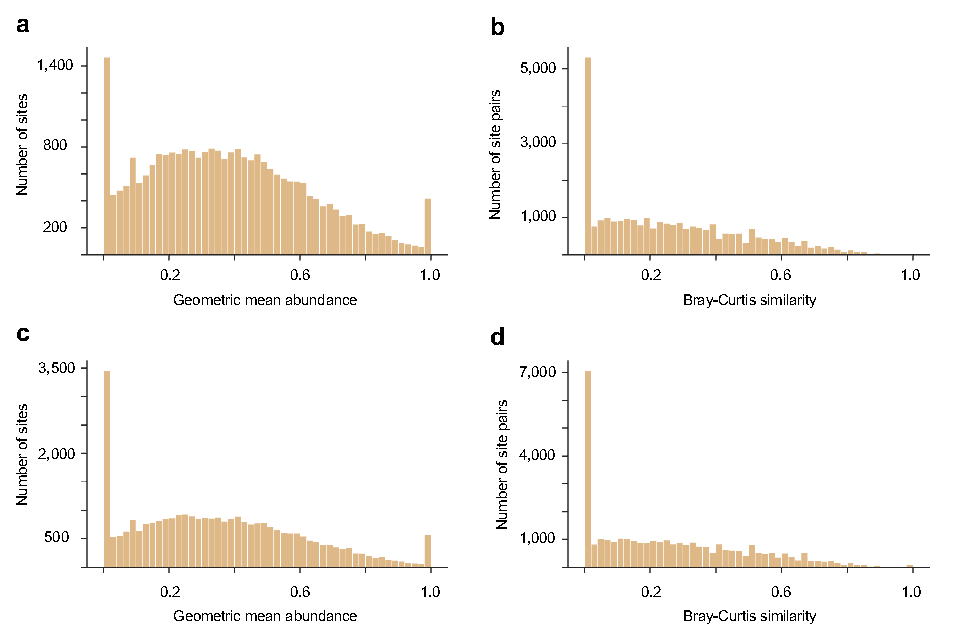
\includegraphics[width=0.95\linewidth]{figures/extended/response_variable_distr.pdf}
    \caption{
    \textbf{Response variable distributions.}
    Data distribution of the response variables for the alpha and beta diversity models. Alpha diversity is measured as the geometric mean abundance per site (for the SBM model, \textbf{a}) or per site and taxa (BTM model, \textbf{c}). Beta diversity is measured as the Bray-Curtis similarity between pairs of sites and reference sites within a study (for the SBM model, \textbf{b}), or between taxa at pairs of sites (BTM model, \textbf{d}).
    }
    \label{fig:response_data_distr}
\end{extendedfigure}
\newpage

\begin{extendedfigure}[H]
    \centering
    \noindent\rule{\linewidth}{0.4pt}\par\vspace{6pt}
    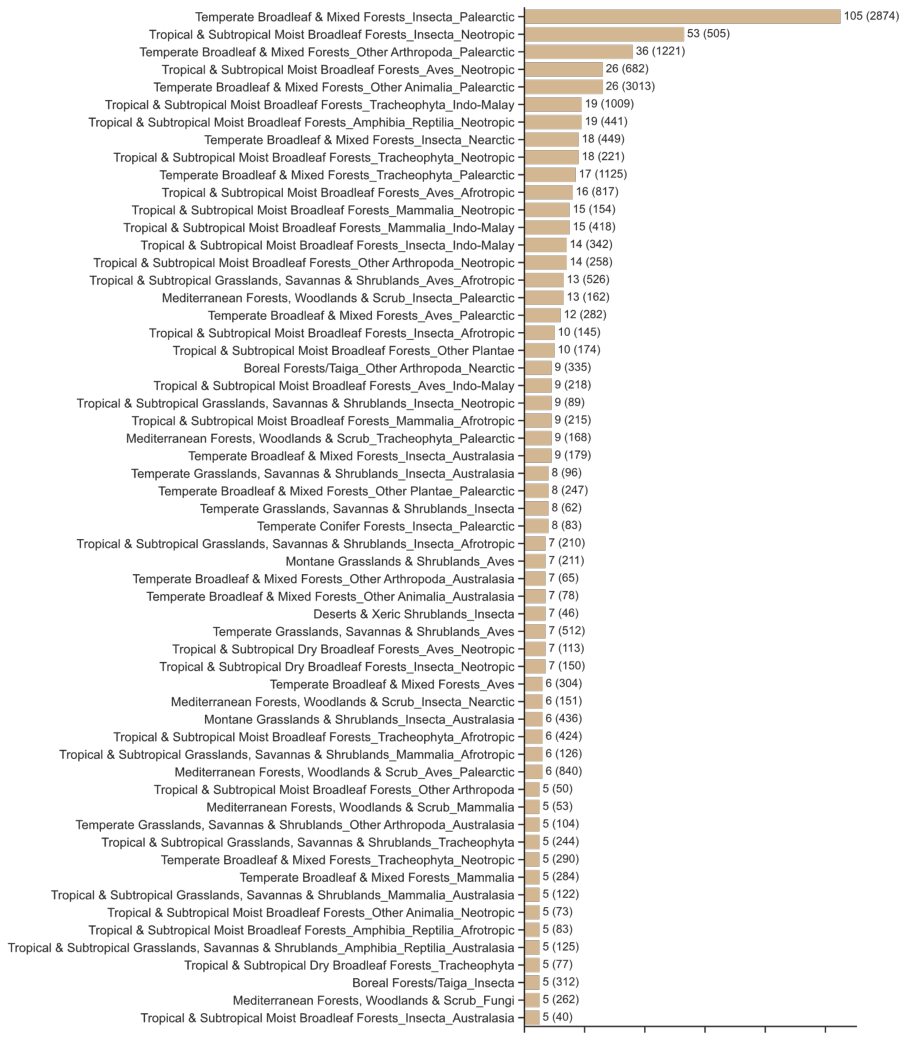
\includegraphics[width=0.95\linewidth]{figures/extended/hierarchical_groups.pdf}
    \caption{
    \textbf{Hierarchical groups in the BTMs.}
    Number of source studies and sampling sites (in parenthesis) in each final biogeographic-taxonomic group included in the BTMs. Some groups are at the biome-taxonomy-realm level, while others have been rolled up to the biome-taxonomy level. Groups that were rolled up to the overall population mean level have been excluded.}
    \label{fig:hierarchical_groups}
\end{extendedfigure}
\newpage

\begin{extendedfigure}[H]
    \centering
    \noindent\rule{\linewidth}{0.4pt}\par\vspace{6pt}
    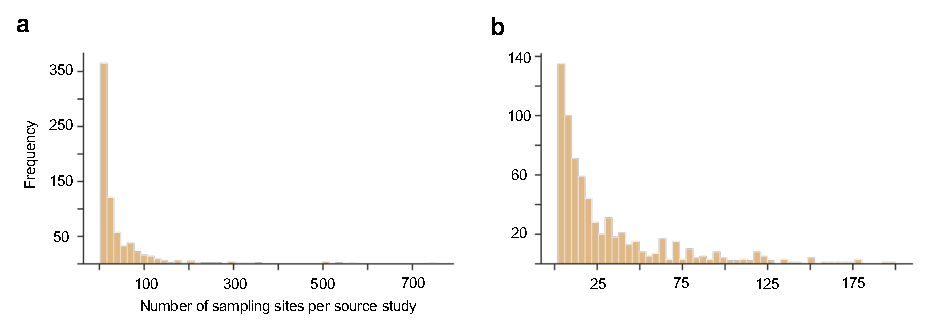
\includegraphics[width=0.95\linewidth]{figures/extended/sites_per_study.pdf}
    \caption{
    \textbf{Sampling sites per study.}
    \textbf{a}, Distribution over the number of sampling sites per source study in the analysis. \textbf{b}, The same distribution but capped at 200 sites, to better show the distribution of the majority of source studies. In the data, 18.8\% of studies have 5 sites or less, while 60.9\% have 25 or less.}
    \label{fig:sites_per_study}
\end{extendedfigure}


\end{document}
